%%%%%%%%%%%%%%%%%%%%%%%%%%%%%%%%%%%%%%%%%%%%%%%%%%%
%
%  New template code for TAMU Theses and Dissertations starting Fall 2012.  
%  For more info about this template or the 
%  TAMU LaTeX User's Group, see http://www.howdy.me/.
%
%  Author: Wendy Lynn Turner 
%	 Version 1.0 
%  Last updated 8/5/2012 
%
%%%%%%%%%%%%%%%%%%%%%%%%%%%%%%%%%%%%%%%%%%%%%%%%%%%  
%%%%%%%%%%%%%%%%%%%%%%%%%%%%%%%%%%%%%%%%%%%%%%%%%%%%%%%%%%%%%%%%%%%%%%
%%                           SECTION III
%%%%%%%%%%%%%%%%%%%%%%%%%%%%%%%%%%%%%%%%%%%%%%%%%%%%%%%%%%%%%%%%%%%%%
\chapter{\uppercase{STRUCTURAL ANALYSES}}  
\label{section:structural_analyses}

This chapter presents analyses of electro-active structures under several loading histories.
The constitutive equations that were introduced in the previous chapters are used for the active materials.
Two types of smart structures are studied, which are smart multi-layered beams and active fiber composites.
The smart beams consist of layers of piezoelectric and inactive materials.
Through thickness electric fields are prescribed in order to create bending in the beams.
Analytical solutions of the deflections of smart beams with time dependent and electro-mechanical coupling effect are presented.
The analytical solutions are also compared to the results obtained from finite element analyses and experiments.
The active fiber composite comprises of unidirectional fibers placed in a polymeric matrix.
Electrode fingers are attached to the top and bottom surfaces of the composite.
In this study, a representative unit cell model is considered for the active fiber composite and the overall electro-mechanical response of the composite is examined. \\

\section{Analyses of Smart Beams}
Analytical and numerical solutions of the time-dependent electro-mechanical coupled deformations of piezoelectric multi-layered composite beams are presented. 
The Laplace transform method is used to obtain the analytical solutions while finite element method is considered for the numerical solutions.
The results from the analytical solutions are compared with the experimental data and finite element solutions.
Several parametric studies are also conducted in order to study the time-dependent electro-mechanical behavior of the composites.
\\


\begin{figure}
\centering
\includegraphics[trim = 0mm 70mm 10mm 60mm,
clip,width=7.0in]{./chap_4_structural_analyses/pdf_beam/PVDF_beam_geometry.pdf}
\caption{Substrated bimorph beam geometry}
\label{fig:PVDF_beam_geometry}
\end{figure}

\subsection{Governing Equation for Electro-Active Beams}
The analyses presented here are suitable for multi-layered slender beams undergoing small deformation gradients.
Figure \ref{fig:PVDF_beam_geometry} illustrates an example of a multi-layered active beam.
This beam has three layers, two active layers at the top and bottom and one substrate (inactive) layer in the center.
There are electrodes on the surfaces of active layer.
An electric field is obtained to these active layers by applying an electric potential difference to the electrodes.
In order to describe the various beam theories, the following coordinate system is introduced.
The
 $x_1$-coordinate is taken along the length of the beam,
 $x_2$-coordinate is taken along the width of the beam, and the
 $x_3$-coordinate along the thickness (the height) of the beam.
According to this coordinate system the loading and geometry are such that the displacements
 $(\bar {u_1}, \bar {u_2}, \bar {u_3})$ along the coordinates axis
 $( {x_1}, {x_2},  {x_3})$ are independent of $x_2$.
Moreover, it is assumed that displacements in the width of the beam $\bar {u_2}$ is zero.
For the beam analyses, the field variables are:
stress $\sigma_{11}$ and
strain $\varepsilon_{11}$ along the longitudinal axis of the beam,
electric field $E_3$ and electric flux (displacement) $D_3$ through the thickness of the beam.
Strain and electric field are taken as the independent variables.
The corresponding stress and electric displacement field for a linear electro-mechanical response is expressed as:

\begin{equation}
\begin{aligned}
&\sigma_{11}=C_{1111} \varepsilon_{11}-e_{311} E_{3} \\
&D_3=e_{311} \varepsilon_{11}+\kappa_{33}^\varepsilon E_{3}
\end{aligned}
\label{stress_1D_const_eqn_beam:EQN}
\end{equation}
where $C_{1111}$ is the elastic stiffness measured at constant electric field,
$e_{311}$ is the piezoelectric constant, and $\kappa_{33}^\varepsilon$ is the dielectric coefficient at constant strain.

The above constitutive model is used for the static response of piezoelectric material.
This study deals with time dependent response of active composite beams with nonlinear electro-mechanical behavior.
The following constitutive relations for the time-dependent-electro-elastic deformation of solids
 (see chapter \ref{section:chap_02_constitutive_model_for_polarization_switching}) is used for the piezoelectric composite beams shown in figure \ref{fig:PVDF_beam_geometry} :

\begin{equation}
\begin{aligned}
\sigma_{11}(t)=
&\int_{0^-}^t
K^C(t-s)\frac{\partial \sigma_{11}}{\partial\varepsilon_{11}} (\varepsilon_{11}(s))\frac{\partial {\varepsilon}_{11}(s)}  {\partial s} ds +\\
&\int_{0^-}^t
K^e (t-s) \frac{\partial \sigma_{11}}{\partial E_{3}}(E_3(s))  \frac{\partial {E}_{3} (s)}  {\partial s} ds
\\
D_3(t)=
&\int_{0^-}^t
K^{e}(t-s)
\frac{\partial D_{3}}{\partial \varepsilon_{11}}(\varepsilon_{11}(s))
\frac{ \partial {\varepsilon}_{11}(s)}  {\partial s}  ds + \\
&\int_{0^-}^t
K^{\kappa}(t-s) \frac{\partial D_{3}}{\partial E_{3}}(E_3(s))  \frac{\partial {E}_{3} (s)}  {\partial s} ds
\end{aligned}
\label{visco_stress_1D_const_eqn_beam:EQN}
\end{equation}
This is a one dimensional version of the 3D constitutive equation that is suitable for beam analyses.
$K^{\kappa}(t), K^e(t), K^C(t)$ are the normalized time dependent kernels.
The time kernels in this constitutive equation can be expressed in terms of Prony series as discussed in chapter \ref{section:chap_02_constitutive_model_for_polarization_switching}. 
A beam is defined as a structural element that is predominantly under bending. 
Three beam theories are considered which are the classical Euler-Bernoulli beam theory, Timoshenko beam theory, and higher order beam theory.
The Euler-Bernoulli beam theory is followed, in which the deformation due to the transverse shear is ignored.
The displacements fields are defined in terms of only two unknown variables, for the transverse displacement and axial displacement:

\begin{equation}
\begin{aligned}
& \bar {u_1} (x_1,x_2,x_3,t)=u_1 (x_1,t)-x_3  \frac{\partial u_3 (x_1,t)} {\partial x_1} \\
& \bar {u_2} (x_1,x_2,x_3,t)=0 \\
& \bar {u_3} (x_1,x_2,x_3,t)=u_3 (x_1,t)
\end{aligned}
\label{eluer_beam:EQN}
\end{equation}
where  $(u_1,u_3)$ are the displacements along the coordinates axis $({x_1}, {x_3})$ measured at the neutral axis.
The Euler-Bernoulli beam theory is valid when the beams are slender enough.
On the other hand if the shear stress in the thickness direction of the beam contributes to the lateral deflection, Timoshenko beam theory is used.
The Timoshenko beam theory assumes a constant shear stress in the thickness of beam and the normal axis to the neutral axis of the beam can rotate with respect to the center line.
This will introduce a new degree of freedom and a new unknown function due to the additional rotation:

\begin{equation}
\begin{aligned}
& \bar {u_1} (x_1,x_2,x_3,t)=u_1 (x_1,t)+x_3  \psi_2(x_1,t)  \\
& \bar {u_2} (x_1,x_2,x_3,t)=0 \\
& \bar {u_3} (x_1,x_2,x_3,t)=u_3 (x_1,t)
\end{aligned}
\label{timoshenko_beam:EQN}
\end{equation}

In the Timoshenko beam theory, the unknown function $\psi_2(x_1,t)$ is a measure of rotation of the beam.
The axial beam displacement ${u_1}$ and transverse displacement field of the beam ${u_3}$ have the same meaning as equation (\ref{eluer_beam:EQN}).
It can be shown by the elasticity solution that the through thickness stress of the beam is quadratic with respect to the transverse coordinate $x_3$ while the Timoshenko beam theory assumes a constant shear stress through the thickness.
In order to correct this inconsistency the shear energy of beam is related to the shear energy of the Timoshenko beam by a constant called shear correction factor.
This constant depends on the geometry of the cross section of the beam and it affects the accuracy of the solutions.
The higher order beam theory is introduced to account for the quadratic distribution of the shear through the thickness of the beam and relax the need for the shear correction factor.


The higher order beam theory uses the same number of degrees of freedom as the Timoshenko beam and therefore, the same number of unknowns of the displacement field.
Using the fact that, the shear stress is zero in the upper and bottom surface of the beam, the quadratic distribution of the shear stress in the thickness is defined.
The displacement field of the theory is defined based on three unknown as in the Timoshenko beam theory:

\begin{equation}
\begin{aligned}
& \bar {u_1} (x_1,x_2,x_3,t)=u_1 (x_1,t)+x_3  \phi_2(x_1,t) +\alpha x_3^3(\phi_2(x_1,t)+\frac{\partial u_3 (x_1,t)} {\partial x_1}) \\
& \bar {u_2} (x_1,x_2,x_3,t)=0 \\
& \bar {u_3} (x_1,x_2,x_3,t)=u_3 (x_1,t)
\end{aligned}
\label{higher_order_beam:EQN}
\end{equation}

By applying stress free conditions on the top and bottom surface of the beam value of $\alpha$ is found to be  $-4/3h^2$ \cite{Wang2000}.
Here $\phi_2(x_1,t)$ is defined as the slope of the normal line measured from the neutral axis.
It can be seen that the normal line in the beam is not straight anymore and it is defined as a cubic function.
The non zero strain component for the displacement defined in the beam equations (\ref{eluer_beam:EQN}-\ref{higher_order_beam:EQN}) are:
\begin{equation}
\begin{aligned}
& \varepsilon_{11} (x_1,x_3,t)=\frac{\partial    \bar {u_1} (x_1,x_3,t) } {\partial x_1} - x_3 \frac{\partial^2 \bar{ u_3} (x_1,x_3,t) } {\partial x_1^2} \\
& 2  \varepsilon_{13} (x_1,x_3,t)=\frac{\partial \bar {u_3} (x_1,x_3,t) } {\partial x_1} + \frac{\partial       \bar{ u_1} (x_1,x_3,t)} {\partial x_3}
\end{aligned}
\label{_strain_beam:EQN}
\end{equation}
This strain formulation can be used for each of the above beam theories.
It is worth noting that for the Euler-Bernoulli beams theory $\varepsilon_{13}$ is zero.
The higher order beam theories can incorporate the effect of shear in the thickness of the beam.
In the case of active composite beams are subjected to electric field through thickness with no transverse mechanical loading, the transverse shear deformation is insignificant.
As a result, using the Timoshenko or higher order beam theories for predicting the deflection gives the same result as the Euler-Bernoulli beam theory.
Therefore, in this study the Euler-Bernoulli beam theory is used for for the smart beams.



Using the variational method, the equilibrium equations for the beam model are determined.
The external axial force $N_{11} (x_1,t)$ and bending moment  $M_{11} (x_1,t)$ are given as:

\begin{equation}
\begin{aligned}
& N_{11} (x_1,t)=\int_{x_2,x_3}\sigma_{11} (x_1,x_3,t)dx_2 dx_3 \\
& M_{11} (x_1,t)=\int_{x_2,x_3}x_3 \sigma_{11} (x_1,x_3,t)dx_2 dx_3 \\
\end{aligned}
\label{resultant_strain_beam:EQN}
\end{equation}
The equilibrium equations for the beam bending are:

\begin{equation}
\begin{aligned}
& \frac{\partial N_{11} (x_1,t)}{\partial x_1}=f(x_1,t) \\
& -\frac{\partial^2 M_{11} (x_1,t)}{ \partial x^2_1}=q(x_1,t)\\
\end{aligned}
\label{equilibrium_resultant_strain_beam:EQN}
\end{equation}
where
$f(x_1,t)$ and $q(x_1,t)$  are  the
distributed axial and transverse loads respectively.
\\

\subsection{Responses of 3-Layered Active Beam Under Constant Electric Field}
\label{section:piezo_beam_static_elastic_solution}
This section presents solution for the analyses of 3-layered active beams using the Euler-Bernoulli beam theory.
First, the response of the beam neglecting the time dependent effect is obtained.
This result is used to verify the finite element formulation and also used to develop the time dependent solution by using the Laplace transform method.
The analytical method that is discussed here is then extended to time dependent and nonlinear electro-mechanical formulation.


Consider a bimorph beam with a thickness $h$ as shown in figure \ref{fig:PVDF_beam_geometry}.
The beam consists of two layers of piezoelectric materials with thickness $h_p/2$ each.
A substrate layer between these two layers of piezoelectric has a thickness $h_s$.
In practice there are electrodes placed between layers and also on the top and bottom parts of the beam in order to prescribe electric field inputs.
If the electric potential $V$ is applied to top and bottom electrodes, the
 piezoelectric layers will be subjected to electric field $E_3=2V/h_p$.
The applied electric field in each layer can be either positive or negative depending on the direction of electric potential applied.
Regardless of the sign of the applied potential the direction of the formed electric fields on the top and bottom layers are opposite to each other in order to create bending.
Since the electrode layer is very thin, its effect on the overall response of the beam is disregarded.
The total thickness of the beam is $h=h_p+h_s$ as shown in figure \ref{fig:PVDF_beam_geometry}. 
Using the equilibrium equation in (\ref{equilibrium_resultant_strain_beam:EQN}), and the linear electro-mechanical constitutive model
 presented in equation (\ref{stress_1D_const_eqn_beam:EQN}) the axial force and bending moments are:

\begin{equation}
\begin{aligned}
 N_{11} (x_1)=& \left( w{\it C_p} {\it h_p}+w{\it C_s} {\it h_s} \right) {\it u_1} \\
 M_{11} (x_1)=& \left( -  {  C_p} {{  h_p}}^{2}{  h_s}/4- {C_p}
{h_p} {{  h_s}}^{2}/4- {C_p} h_p^3/12- { C_s} {{h_s}}^{3} /12 \right)w
\frac{\partial^2 u_3 (x_1,t)} {\partial x_1^2}-  \\
& w e E_3 ( {h_p} {h_s}/2- {h_p}^{2}/4)
\end{aligned}
\label{EQN:stress_resultant_integration_definistion}
\end{equation}
where
$w$ is the width of the beam.
A simplified notation for the material parameters is considered here.
For the piezoelectric layer the stiffness and piezoelectric constants are $C_{1111}=C_p$, $e_{311}=e$ respectively.
For the elastic substrate the properties are $C_{1111}=C_s$ and $e_{311}=0$.
The effect of the electric displacement on the strain is ignored.
If the beam shown in figure \ref{fig:PVDF_beam_geometry} is clamped at the left end, the boundary conditions are as follows:
\begin{equation}
u_1(0)=u_3(0) =\frac{ \partial u_3(0) } {\partial x_1}=0
\label{Eqn:clamped_beam_boundary_conditions}
\end{equation}
Then, for a beam with no transverse loading the deflection of the beam is:
\begin{equation}
u_3
(x_1)=\frac{1}{2}\frac{3 e E h_p (h_p+2h_s)}{C_p h_p^3+3
C_p h_p^2 h_s+3C_p h_p h_s^2+C_s h_s^3} x_1^2
\label{EQN:deflecction} 
\end{equation}


The above analyses is extended for the time dependent constitutive equation of active composite beams.
The time dependent electro-mechanical constitutive piezoelectric layers and linear visco-elasticity is considered for the substrate.
A closed-form solution for the deformations of the active beam is presented.
The time dependent response of the beam is obtained by using the Laplace transform method.
Consider the beam geometry as shown in figure \ref{fig:PVDF_beam_geometry},
 with the constitutive equation (\ref{visco_stress_1D_const_eqn_beam:EQN}) for the piezoelectric layers of the beam.
The stress in the piezoelectric layers is additively decomposed into the mechanical and electro-mechanical stresses:
\begin{equation}
\sigma_{11}=\sigma_{11}^m+\sigma_{11}^e
\end{equation}
where
\begin{equation}
\begin{aligned}
\sigma_{11}^m&=\int_{0^-}^t
K^C(t-s)\frac{\partial \sigma_{11}}{\partial\varepsilon_{11}} (\varepsilon_{11}(s))  \frac{\partial {\varepsilon}_{11}(s)}{\partial s}ds\\
\sigma_{11}^e&=\int_{0^-}^t
K^e (t-s) \frac{\partial \sigma_{11}}{\partial E_{3}}(E_3(s)) \frac{\partial {E}_{3} (s)}{\partial s} ds
\end{aligned}
\label{eqn:history_dependent_stress_and_strain}
\end{equation}

The mechanical stress is considered to be linear and elastic,
which for the host structure and active layer are $\sigma_{11}^m=C_s \varepsilon_{11}$ and $\sigma_{11}^m=C_p \varepsilon_{11}$.
The stress due to the electro-mechanical coupling is defined as a polynomial function of the electric field in order to include the effect of high electric fields.



The Laplace transform is used to transform the equations from time domain to the Laplace variable domain.
The derivatives with respect to time will be expressed as polynomials with respect to the Laplace variable.
The constitutive equation (\ref{eqn:history_dependent_stress_and_strain}) for beam is presented in the Laplace form as:

\begin{equation}
\mathcal{L} \left[ \sigma_{11}(t) \right]=a  C_p \mathcal{L} \left[ K^C(t) \right] \mathcal{L} \left[ \varepsilon_{11}(t) \right]
\end{equation}
where $\mathcal{L}$ is the Laplace transform and $a$ is the transform variable.
In the same manner the Laplace transform for the electro-mechanical stress $\sigma_{11}^e$ is defined.

\begin{equation}
\mathcal{L} \left[ \sigma_{11}^e(t) \right]=\mathcal{L} \left[
\int_{0^-}^t
K^e (t-s) \frac{\partial \sigma_{11}}{\partial E_{3}}(E_3(s))  \dot{E}_{3} (s)ds
\right]
\label{EQN:Laplace_stress_coupling}
\end{equation}
Since the electric field is known, the explicit definition of the electro-mechanical coupling stress in the Laplace domain is obtained using equation (\ref{EQN:Laplace_stress_coupling}).
The Laplace transform turns the time dependent integral equation into an algebraic equation.


% In dealing with nonlinear and time dependent response we are dealing a differential equation for displacement field with respect to coordinates and also integral equation with respect to time.
% Laplace transform will seperate the time dependent integral equation and turn it into polynomila with respect to laplace variable so we can solve the ordinary equation with respect to coordinate such as static case.
The differential equation for the displacement with respect to spatial variables are given in Equations (\ref{equilibrium_resultant_strain_beam:EQN}) and (\ref{resultant_strain_beam:EQN}).
The axial force and bending moment in the Laplace domain are:

\begin{equation}
\begin{aligned}
&\bar{N}_{11} (x_1,a)=\int_{x_2,x_3} \bar{\sigma}_{11} (x_1,x_3,a) dx_2 dx_3 \\
&\bar{M}_{11} (x_1,a)=\int_{x_2,x_3} x_3 \bar{ \sigma}_{11} (x_1,x_3,a) dx_2 dx_3 \\
\end{aligned}
\label{EQN:laplac_resultant_strain_beam}
\end{equation}
where the upper bar means the function in Laplace domain.
The equilibrium equations are:

\begin{equation}
\begin{aligned}
& \frac{\partial \bar{N}_{11} (x_1,a)}{\partial x_1}=\bar{f}(x_1,a) \\
& -\frac{\partial^2 \bar{M}_{11} (x_1,a)}{ \partial x^2_1}=\bar{q}(x_1,a)\\
\end{aligned}
\label{EQn:Laplace_equilibrium_resultant_strain_beam}
\end{equation}
It is noted that the applied transverse and axial boundary conditions should be defined in the Laplace domain.
The Laplace transform should also be performed for the time dependent boundary conditions.
Solving the differential equations presented in equation (\ref{EQn:Laplace_equilibrium_resultant_strain_beam}) will result in transverse deflection in Laplace space $\bar{u}_3(x_3,a)$.
The inverse of the Laplace transform gives the function in time domain:

\begin{equation}
u_3(x_3,t) =\mathcal{L}^{-1} \left[ \bar{u}_3(x_3,a) \right]
\label{eqn:inverse_laplace_of_transverse_displace_ment}
\end{equation}
\\
\begin{figure}
\centering
\includegraphics[trim = 0mm 60mm 10mm 60mm,
clip=true,width=7.0in]{./chap_4_structural_analyses/pdf_beam/bimorph_PVDF_beam_geometry.pdf}
\caption{Bimorph PVDF beam geometry and placement of electrodes}
\label{fig:bimorph_PVDF_beam_geometry}
\end{figure}



\subsection{Numerical Validation}
This section compares the result from the analytical solutions to the finite element analyses.
The objective of this study is to validate the results from finite element analyses.
The experimental data published in literature are also used to validate the analytical and finite element solutions.

An experiment that has been done on a PVDF bimorph is first simulated.
The bimorph beam is subjected to a constant electric field input.
The PVDF layer is polarized through its thickness direction.
The configuration of the beam is illustrated in figure \ref{fig:bimorph_PVDF_beam_geometry}.
This beam is modeled with the results from equation (\ref{EQN:deflecction}) with $h_s=0$ and $h_p=h/2$.
Figure \ref{fig:bimorph_PVDF_beam_geometry} also illustrates the electrodes that are placed on the top, bottom and middle layers of the beam.
The electric potential is applied to the central electrode, and the top and bottom electrodes are grounded.
This actuation architecture guarantees that the two PVDF layers will be under electric field in the opposite direction, inducing opposite axial stresses to the top and bottom layers and,
allowing for the beam to bend.
The distribution of the electric potential through the thickness of the beam from the finite element analyses is shown in figure \ref{fig:PVDF_beam_geometry_epot_distribution}.
The bending deformation of the bimorph beam is predicted using a linear piezoelectric constitutive equation.
Experimental data reported by \cite{tzou1991distributed} and analytical solutions \cite{raey,franco2000modelling,suleman1995simple} of the tip deflection of the bimorph beam are used for comparisons.
The material properties used for the PVDF are taken from \cite{suleman1995simple} and also \cite{franco2000modelling}.
The Young's modulus $C_p$ or $E_y$ is considered to be $2 GPa$ and the shear modulus is taken $1GPa$.
The electro-mechanical constant for PVDF, in this case, is taken as $e_{311}=e=0.046 C/m^2$.
The dielectric constant or electric dielectric coefficient is taken to be $ k^\varepsilon = 0.1062 \times 10^{-8} F/m$.
The bonding between the different layers in the bimorph beam is assumed perfect;
thus the traction and displacement continuity conditions are imposed at the interface layers.
The beam has a length $L$ of $100mm$, width of $5mm$ and the thickness of the beam is $1mm$.
The middle layer is under 0.5 V.
This results in $1000 V/m$ electric field to each PVDF layer.
The result from the current model is compared with the experiment and also other computational methods, which are presented in Table \ref{table:PVDF_bimorph_numerical_result_static}.
Good comparisons are observed among the results.

\begin{table}
\caption{Numerical Result from Present Model for Deflection of PVDF Bimorph}
\centering
\begin{tabular}{|l|c|r|} \hline
Method  &   &  Tip deflection $\times 10^{-7} m$ \\ \hline
Experiment \cite{tzou1991distributed} &  & 3.15 \\ \hline
Analytical solution & $w(x)=345 x^2$ & 3.45\\ \hline
Plate FEM \cite{franco2000modelling} &  & 3.45 \\ \hline
Beam Finite Difference & 41 nodes & 3.4 \\  \hline
2D FEM present model  & C2D9 elements in 10x4y mesh &3.15 \\  \hline
3D FEM ABAQUS model  & C3D8E elements in 162x10y4z mesh & 2.99\\ \hline
3D FEM ABAQUS model  & C3D20QE elements in 10x1y4z mesh & 3.4414\\ \hline
3D FEM present model  & C3D20 elements in 5x2y2z mesh & 3.455 \\ \hline
\end{tabular}
\label{table:PVDF_bimorph_numerical_result_static}
\end{table}

\begin{figure}
\centering
\includegraphics[trim = 00mm 0mm 00mm 0mm, clip=true,width=7.0in]{./chap_4_structural_analyses/pdf_beam/PVDF_beam_geometry_epot_distribution.png}
\caption{Bimorph PVDF beam electric potential distribution}
\label{fig:PVDF_beam_geometry_epot_distribution}
\end{figure}


The time-dependent behavior of active beams are presented here.  
The Laplace transform method is used for obtaining analytical solutions of the time-dependent electro-elastic beams.
A bimorph beam shown in figure \ref{fig:PVDF_beam_geometry} is subjected to a sinusoidal voltage.
The time dependent kernel function for the electro-mechanical properties in equation (\ref{visco_stress_1D_const_eqn_beam:EQN}) is chosen as $K^e (t)=1+exp(-t)$.
A sinusoidal electric field is applied with frequency of 1 Hz and the amplitude 1 V/mm.
The electro-mechanical coupling effect is considered to be linear, $\frac{\partial \sigma_{11}}{\partial E_{3}}=e_{311}=.046$.

\begin{figure}
\centering 
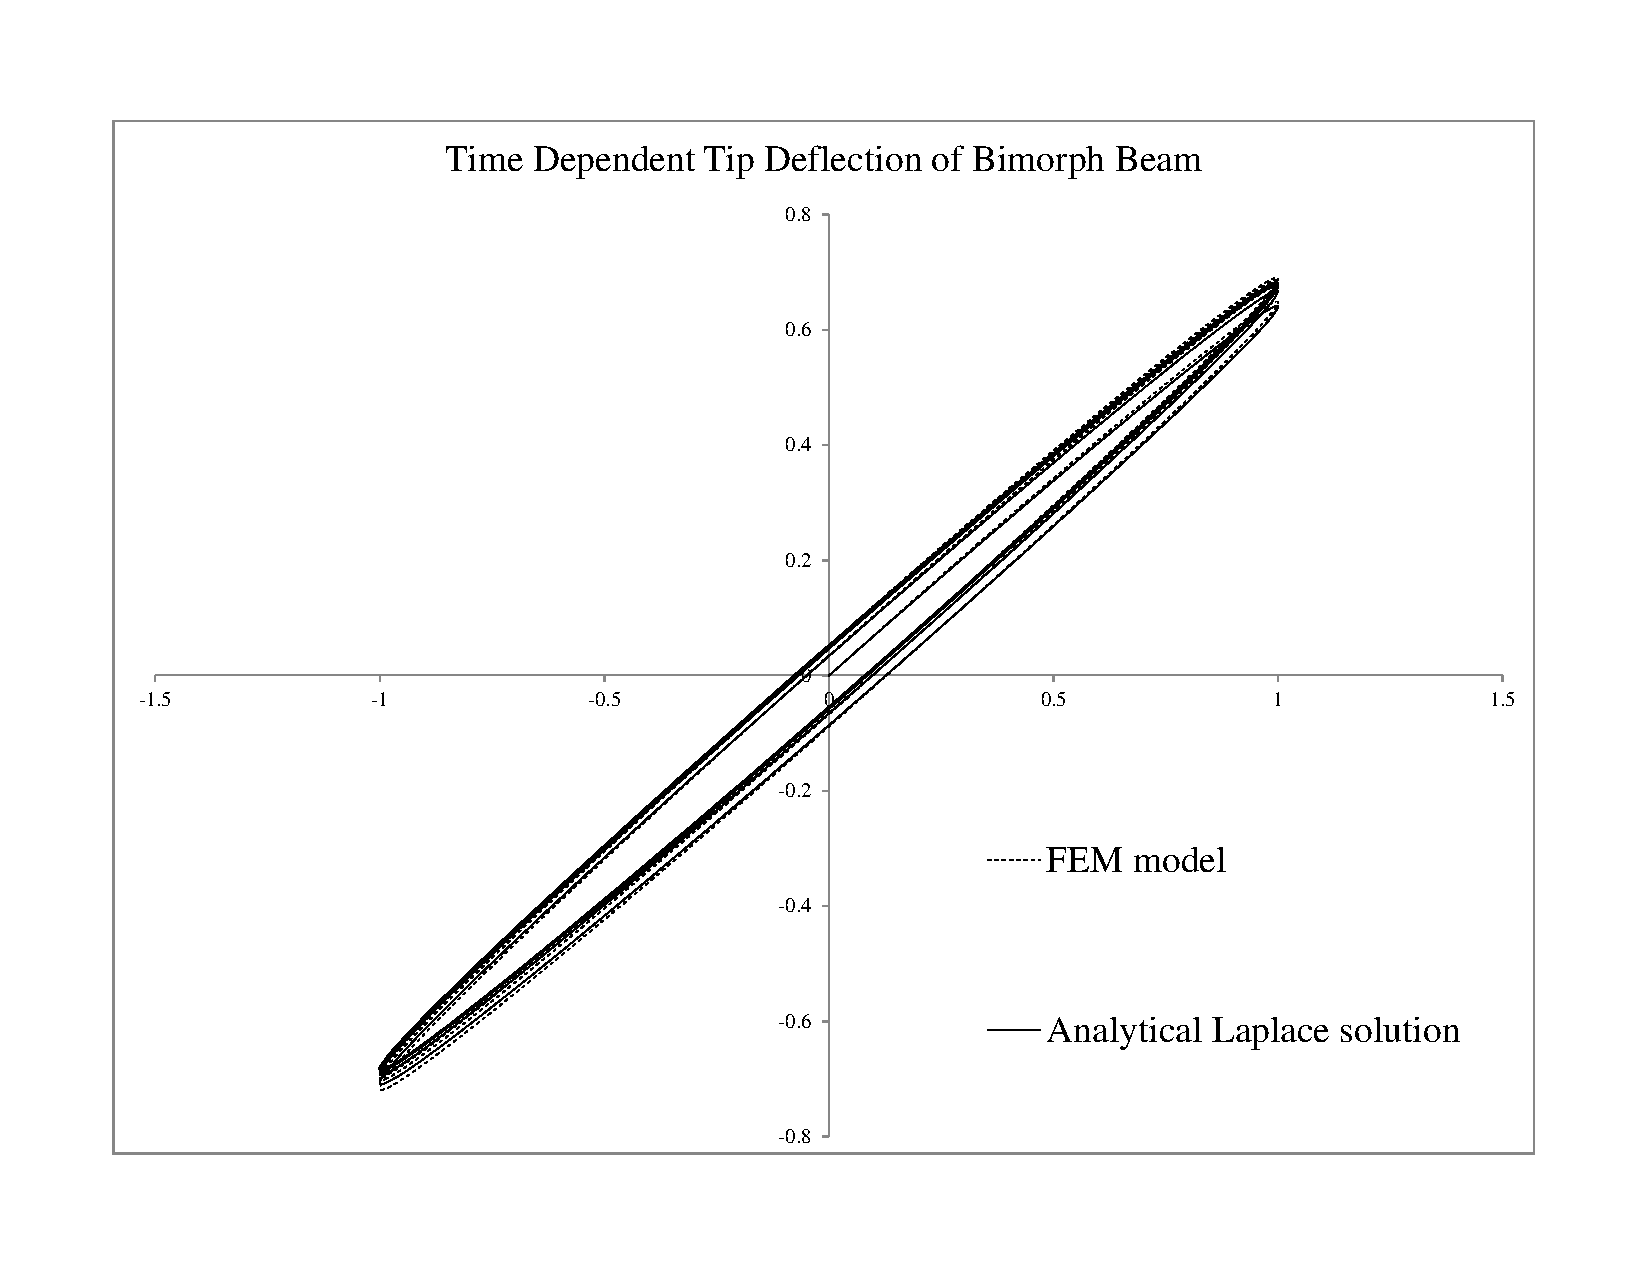
\includegraphics[trim = 0mm 20mm 0mm 20mm,
clip=true,width=7.0in]{./chap_4_structural_analyses/pdf_beam/result_tip_deflection_of_bimorph_beam.pdf}
\caption{Tip deflection of bimorph beam, comparing Laplace solution with numerical recursive method}
\label{fig:result_tip_deflection_of_bimorph_beam}
\end{figure}
Using these values in equations (\ref{eqn:history_dependent_stress_and_strain})-(\ref{eqn:inverse_laplace_of_transverse_displace_ment}) and taking inverse of the Laplace transform,
 the analytical solution for the time dependent deflection of the beam is:

\begin{equation}
\begin{aligned}
u_3(x_1,t)=\frac{A(t)}{B(t)}
\end{aligned}
\label{EQN:PVDF_beam_closed_form_solution}
\end{equation}
where $A(t)$ and $B(t)$ are the solutions of time dependent deformation that is obtained by a commercial computer algebra system, Maple.
For the present case study with the material properties for PVDF and the kernel function that is defined above, are forms for $A(t)$ and $B(t)$ are:

\begin{equation}
\begin{aligned}
&A(t)=A_0 e^{-\lambda_{A_0} t}+A_1 sin(2\pi \lambda_{A_1} t)+A_2 cos(2\pi
\lambda_{A_2} t)
\\
&B(t)=B_0 e^{-\lambda_{B_0} t}+B_1 sin(2\pi \lambda_{B_1} t)+B_2 cos(2\pi
\lambda_{B_2} t)
\end{aligned}
\label{EQN:PVDF_beam_closed_form_solution_functions}
\end{equation}
where the constants for this equation are presented in Table \ref{table:PVDF_bimorph_time_dependent_solution_coefficients}.
The analytical solution is compared with the numerical solution from the recursive finite element analyses.
A 3D quadratic element with 20 nodes is used for finite element.
It is noted that quadratic elements shown to be more accurate in dealing with bending.
% The recursive integration in FE model technique is used to capture the time dependent effect.
The result from analytical solution and finite element analyses are compared in figure \ref{fig:result_tip_deflection_of_bimorph_beam}.
A good match between the Laplace transform method and numerical solution is observed.
This validates the recursive integration algorithm for the linear time-dependent electro-mechanical responses, which are implemented in finite elements.

\begin{table}
\caption{Coefficients for close form time dependent solution of PVDF beam}
\centering
\begin{tabular}{|l|c|c|c|r|} \hline
n & $A_n$ & $B_n$ & $\lambda_{A_n}$& $\lambda_{B_n}$\\ \hline
0 & $-4.462664015\times 10^{19}$ & $8.333333335\times 10^{17}$ & -1.0 & 0.0\\ \hline
1 & $5.678974503\times 10^{20}$ & $1.326291193\times 10^9$ & 1.0 & 1.0\\ \hline
2 & $4.462664015\times 10^{19}$ & $0$ & 1.0 & 0.0 \\ \hline
\end{tabular}
\label{table:PVDF_bimorph_time_dependent_solution_coefficients}
\end{table}

The nonlinear electro-mechanical deflection of an active beam has been experimentally observed by Lin et al. \cite{Li2004959}.
This experiment is used to validate the nonlinear and time dependent closed form solution.
The beam has three layers, two piezoelectric and one metal substrate.
A metallic layer is placed in the middle of the beam with thickness of $h_s=0.0075in$. % or $h_s=127 \mu m$.
The substrate is made of stainless steel and its elastic modulus is taken to be $E_s=C_s=180 GPa$.
Two piezoelectric active layer are placed on the top and bottom of the substrate with thickness of $h_p=0.005in$. % or $h_p=190.5 \mu m$ each.
These layers are activated by electric potential.
The frequency of the excitation is 1Hz and the electric potential is applied with amplitude of 100 V.
The beam's length is $L=1.5 in$. % or $L=38.1 mm$.
The beam's width is $b=0.375 in$. % or $L=952.5 \mu m$.
The stiffness of piezoelectric layers in the longitudinal and transverse direction are reported as $E^L_p=C_p=63 GPa$ and $E^T_p=49 GPa$, respectively.
The electro-mechanical coupling stress is considered to be a nonlinear cubic function of electric field.

\begin{equation}
\sigma^e_{11}(E_3)= e^0_{311}E_3+e^2_{311}E^3_3
\label{EQN:cubic_coupling_stress_three_layer_beam}
\end{equation}
where the constants are taken to $e^0_{311}=14.5 C/m^2$ and $e^2_{311}=-6 pC/m^2$.
Moreover, the time dependent kernel function is taken as
\begin{equation}
K_e(t)=K^e_0+K^e_1exp(-\lambda_1 t )
\label{EQN:time_dependent_kernel}
\end{equation}
where the Prony constants are taken as: $K^e_0=1.7$, $K^e_1=-0.7$ and $\lambda_1=-0.7$.
The beam is constrained to be simply supported.
% They have designed an actuator with four simply supported beam.
% The actuator is designed with two beam at each side.
% Two beam are connected in serial in the way that their central deflection will add up.
The result from the deflection produced by the actuator along with the applied voltage is reported in \cite{Li2004959}.
This comparison is shown in figure \ref{fig:electric_volt_vs_displacement_three_layer_beam}.
The cubic approximation of the electro-mechanical coupling is close enough to the experimental data.
\\

\begin{figure}
\centering
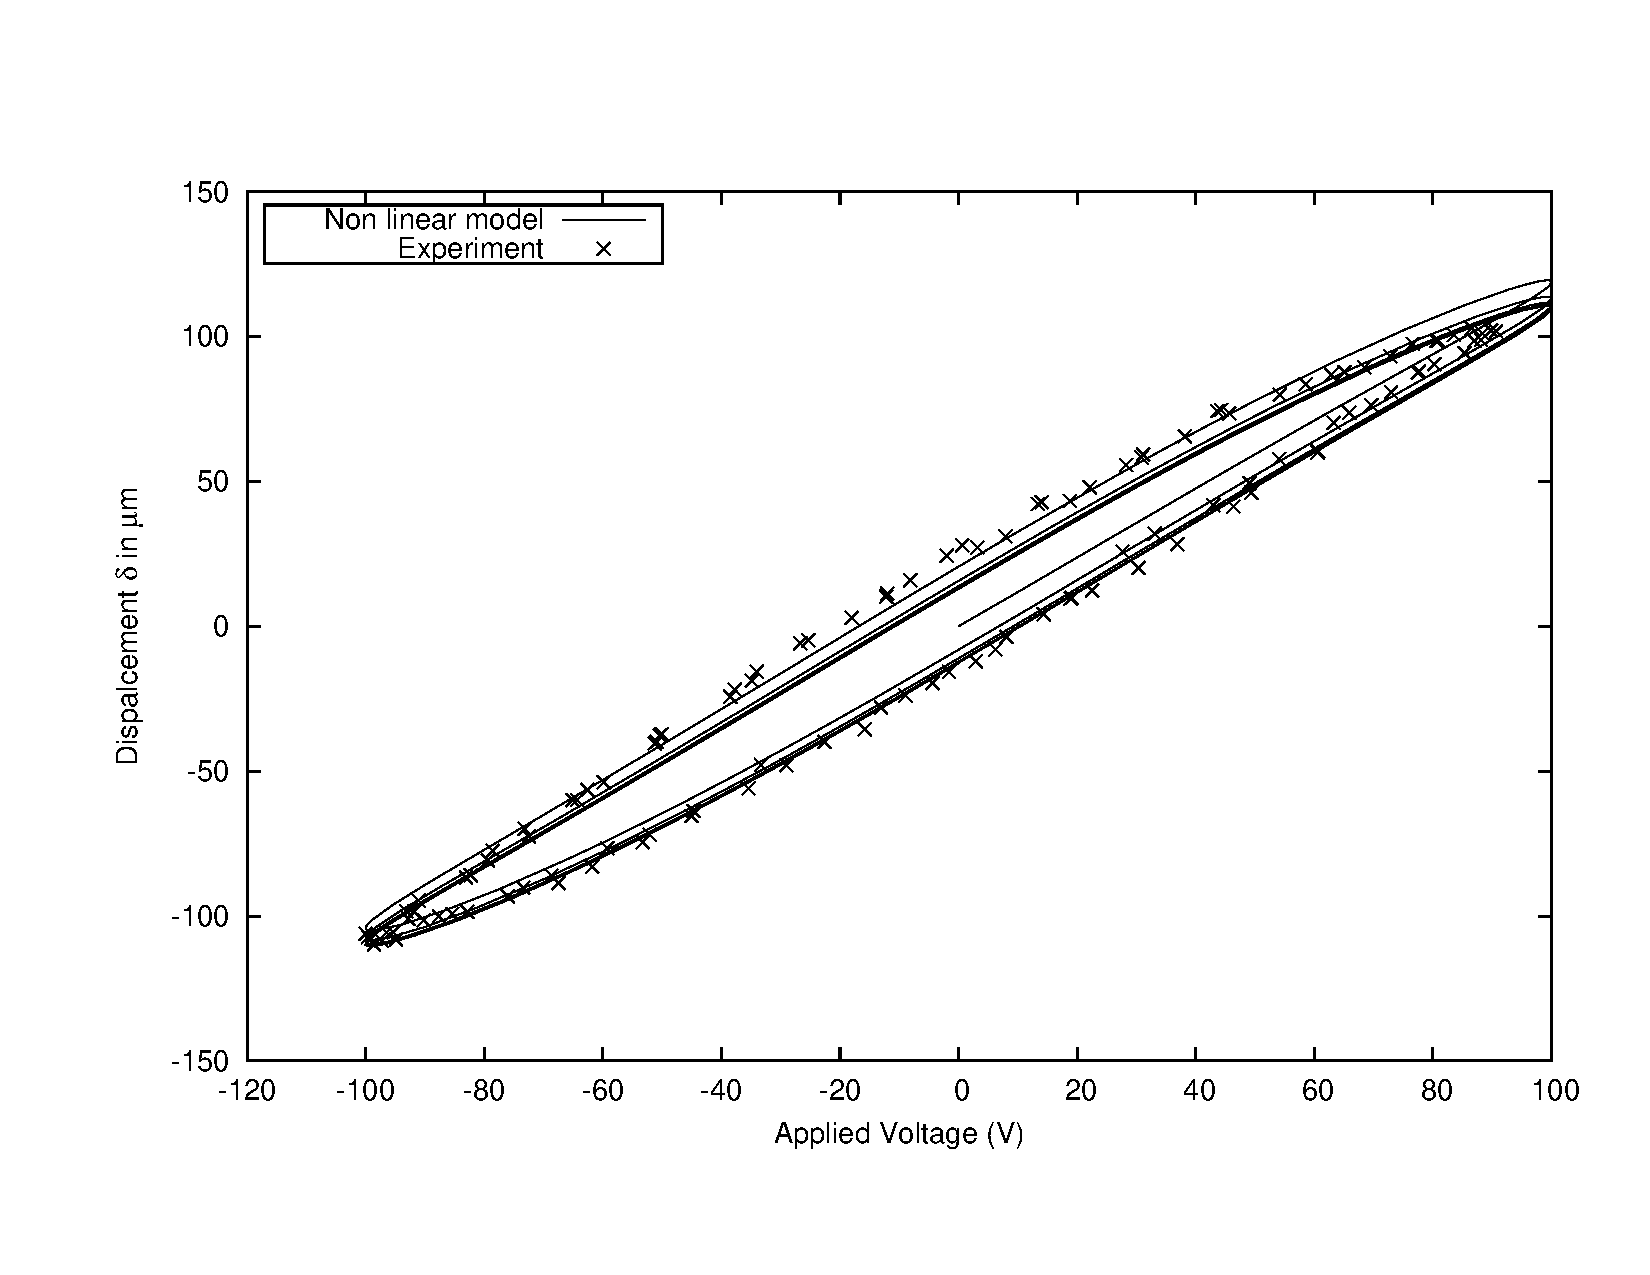
\includegraphics[width=6.0in]{./chap_4_structural_analyses/pdf_beam/electric_field_vs_displacement_three_layer_beam.pdf}
\caption{Experimental result \cite{Li2004959} compared with Laplace solution of an actuator made of three layer active beam}
\label{fig:electric_volt_vs_displacement_three_layer_beam}
\end{figure}


\subsection{Effect of Frequency on the Hysteresis Responses of Active Beams}
The effect of different histories of electric potential inputs is also analyzed.
Consider a bimorph beam consisting of two layers of polarized piezoelectric ceramics and an elastic layer, as shown in figure (\ref{fig:PVDF_beam_geometry}). % TK .
In order to produce a bending deflection in the beam, the two piezoelectric layers should undergo opposite tensile and compressive strains.
The beam is fixed at one end and the other end is left free;
 the top and bottom surfaces are under a traction free condition.
 A potential is applied at the top and bottom surfaces of the beam and the corresponding displacement is monitored.


\begin{figure}
\centering
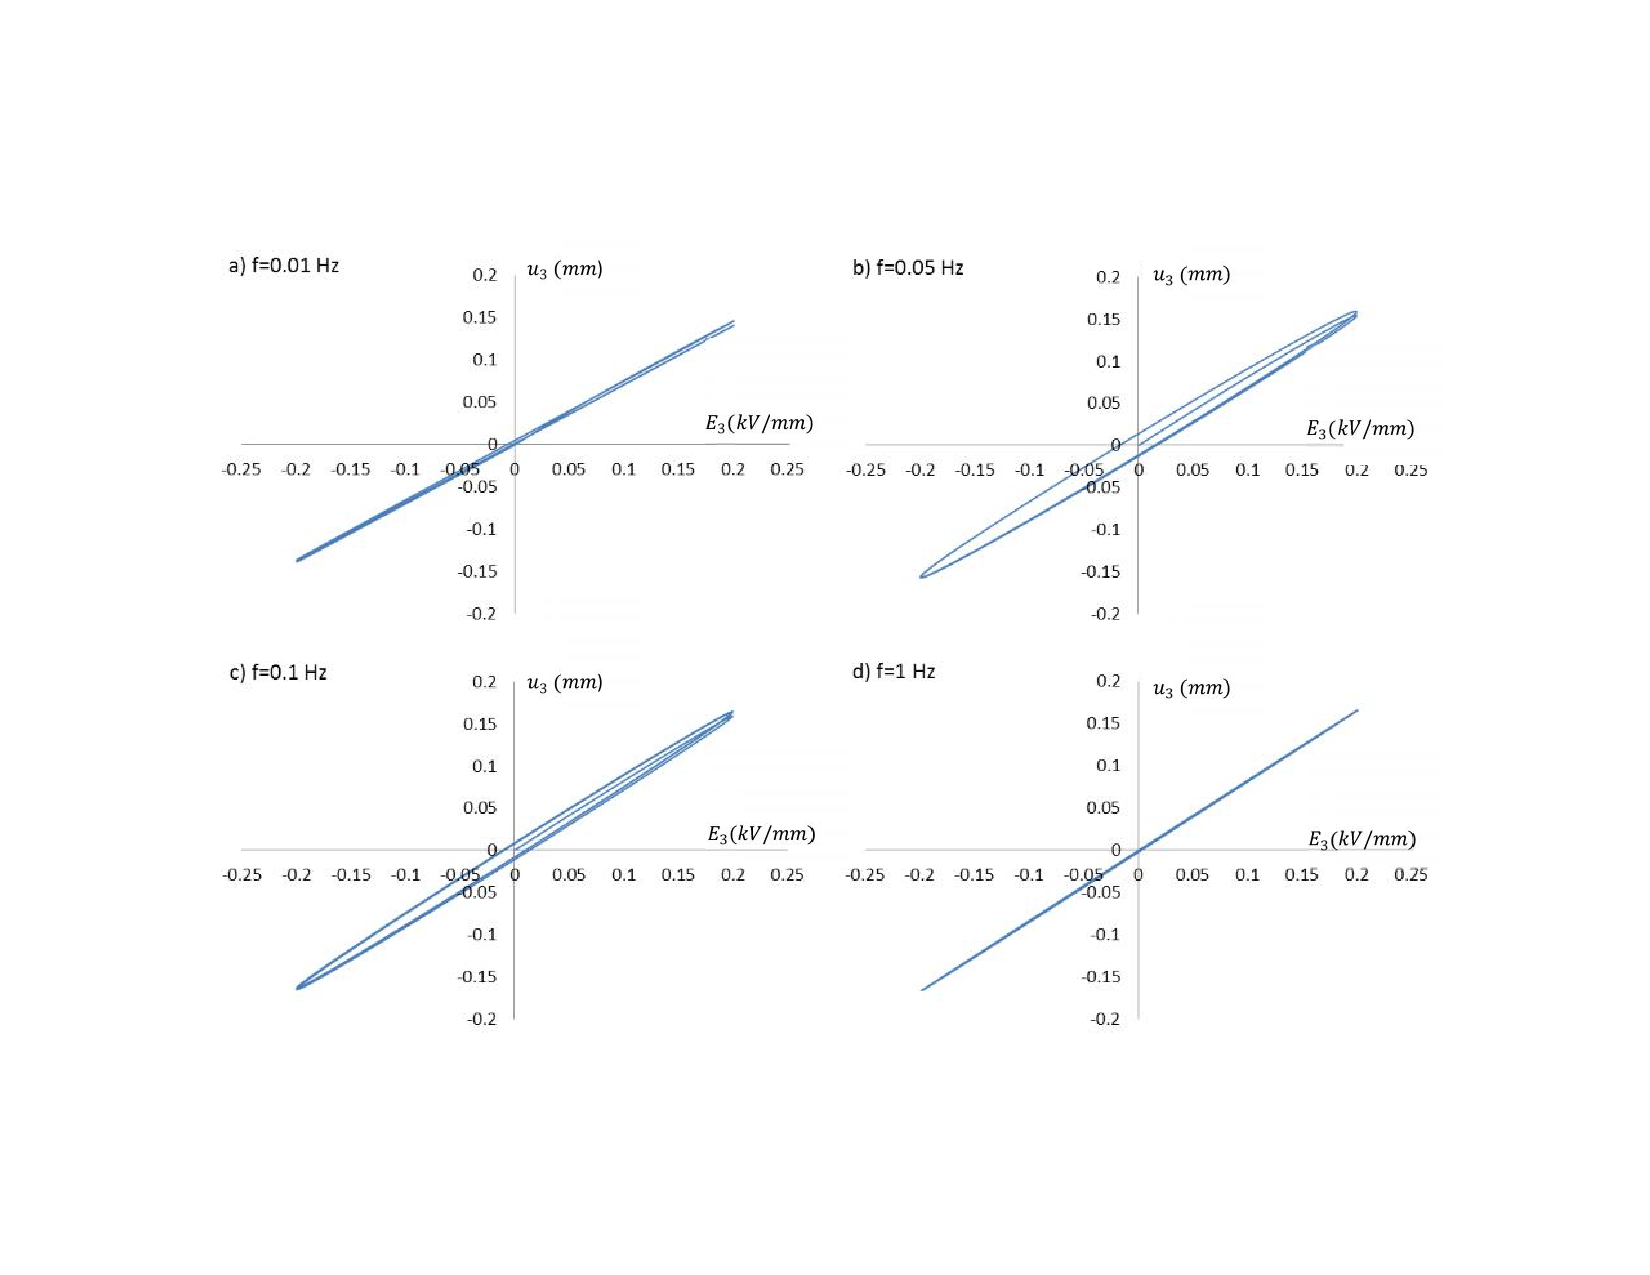
\includegraphics[trim = 0mm 20mm 00mm 40mm,
clip=true,width=6.0in]{./chap_4_structural_analyses/pdf_beam/result_tip_deflection_of_bimorph_beam_frequencies.pdf}
\caption{Tip deflection of bimorph beam, comparing observing effect of frequency of applied electric field}
\label{fig:result_tip_deflection_of_bimorph_beam_frequency}
\end{figure}


A bimorph beam without an elastic layer placed in between the piezoelectric layers is studied as it is shown in (\ref{fig:bimorph_PVDF_beam_geometry}).
It is assumed that the beam is relatively slender so that it is sensible to adopt Euler-Bernoulli beam theory in finding the corresponding displacement of the bimorph beam.
Since a uniform voltage is prescribed on the top and bottom surfaces of the beam, the problem reduces to a pure bending problem.
The beam has a length of 100mm, width of 1mm and the thickness of each piezoelectric layer is 1mm.
The following time-dependent properties of PZT5A are used for the bending analyses.

\begin{equation}
\begin{aligned}
& C_p(t)=90 K^C(t) \, {GPa}      &K^C(t)=1+exp(-0.02 t)/3 \\
& e(t)=-5.35 K^e(t) \, C/m^2 &K^e(t)=1+exp(-0.2 t)/4
\label{Eqn:beam_frequency_material_properties}
\end{aligned}
\end{equation}

A sinusoidal input of an electric potential with various frequencies are applied.
figure \ref{fig:result_tip_deflection_of_bimorph_beam_frequency} illustrates hysteresis response of the bending of the bimorph beam.
The displacements are measured at the free end ($x_1$ =100mm).
When the rate of loading is comparable to the characteristics time,
the effect of time-dependent material properties on the hysteretic response becomes significant,
as shown by the response with frequencies of 0.05Hz and 0.1Hz.
When the rate of loading is relatively fast (or slow) with regards to the characteristics time, i.e. f=0.01Hz and 1Hz,
 insignificant (less pronounced) time-dependent effect is shown, indicated by narrow ellipsoidal shapes.
\\


\section{Large Deformation Analyses}
In this section, large deformation analyses of slender beams is discussed.
We use the bimorph beam geometry that was discussed in the previous example for large deformation analyses.
The geometry of this beam is introduced in figure \ref{fig:bimorph_PVDF_beam_geometry}.
In order to validate the result from finite element model, the closed form formulation for simple case of folding of a biomorph beam is considered.

The Green St. Venant strain induced in the material due to deformations is a quadratic function of the displacement gradient \cite{Lai2009}.
If the deformation is large then the nonlinear term of the strain cannot be disregarded.
The quadratic function for the strain displacement relationship is defined as:

\begin{equation}
\varepsilon_{ij}=\frac{u_{i,j}+u_{j,i}}{2}+\sum_{m=1}^{3} \frac{u_{m,i}u_{m,j}}{2}
\label{EQN:large_displacement_strain}
\end{equation}

Equation (\ref{EQN:large_displacement_strain}) is the more general form of infinitesimal strain theory that is represented in equation (\ref{EQN:Linear_Electric_Field}).
The model is already developed based on nonlinear formulation for multi-functional material.
Therefore, only the terms for strain should be modified in order to capture large deformation.

It is possible to present analytical solutions for folding of beams \cite{Muliana2014}.
The bimorph beam that is considered for large deformation is only under bending due to electric field.
Therefore, the stretch in the beam is neglected.
The strain is assumed linear in stress and the linear constitutive equations presented in equations (\ref{stress_1D_const_eqn_beam:EQN}) and (\ref{resultant_strain_beam:EQN}) are considered for the analyses. 
The internal bending moment of the beam due to the mechanical strain can be presented as \cite{Muliana2014}:

\begin{equation}
M^m_{11}=E_{1} I_{11} \acute{\phi}
\label{EQN:internal_bending_moment_beam}
\end{equation}
where 
$E_{1}$ is the Young modulus and it is same as $C_p$,
$I_{11}$ is the second moment of area that is $h_p^3/12$ in the case of bimorph geometry shown in figure \ref{fig:bimorph_PVDF_beam_geometry},
$\acute{\phi}$ is the curvature of the beam can be presented as $\acute{\phi}=1/r$ where $r$ is the radius of folded shape of beam.      
In case of a complete folding of the beam, the radius of curvature for beam will be $r=\frac{L}{2\pi}$, where $L$ is the length of beam.

The electrical bending moment of beam due to electric field using equations \ref{stress_1D_const_eqn_beam:EQN} and \ref{resultant_strain_beam:EQN} can be presented as:
\begin{equation}
M^e_{11}=\frac{e_p  h_p  V}{2}
\label{EQN:electric_bending_moment_beam}
\end{equation}
There is no other external force or moment is acting on the beam. 
Then, the equilibrium equation in the beam can be satisfied at each point on the neutral axis, thus $M^m_{11}=M^e_{11}$.
 
Considering the mechanical and electrical properties for the PVDF beam the electric potential needed to completely fold the PVDF bimorph beam will be 
\begin{equation}
V_{fold}=\frac{h_p^2 \pi C_p}{3 e_p L}
\label{EQN:electric_potential_to_fold}
\end{equation}
Using the electro-mechanical material properties and geometries of bimorph beam that were discussed before the electric potential for folding the beam is $V_{fold}=455kV$.
This electric potential is applied to the central electrode of the biomorph beam in the finite element analyses.
The result from this analyses is shown in figure \ref{fig:pvdf_beam_folding}.
It can be seen that a complete folding is captured by taking the nonlinear kinematics into account as it is expected from the analytical solution presented.
% This validates the nonlinear geometric analyses of developed multi-functional finite element model.
% It is noted for the sake of consistency with the other simulation reported in the literature only the transverse electro-mechanical coupling is considered in this simulation.
% In the real situation the complete folding of bimorph beam will happen with much lower electric potential due to normal electro-mechanical coupling and incompressibility of polymer that are disregarded in this analyses. 
\\  
 
\begin{figure}
\centering
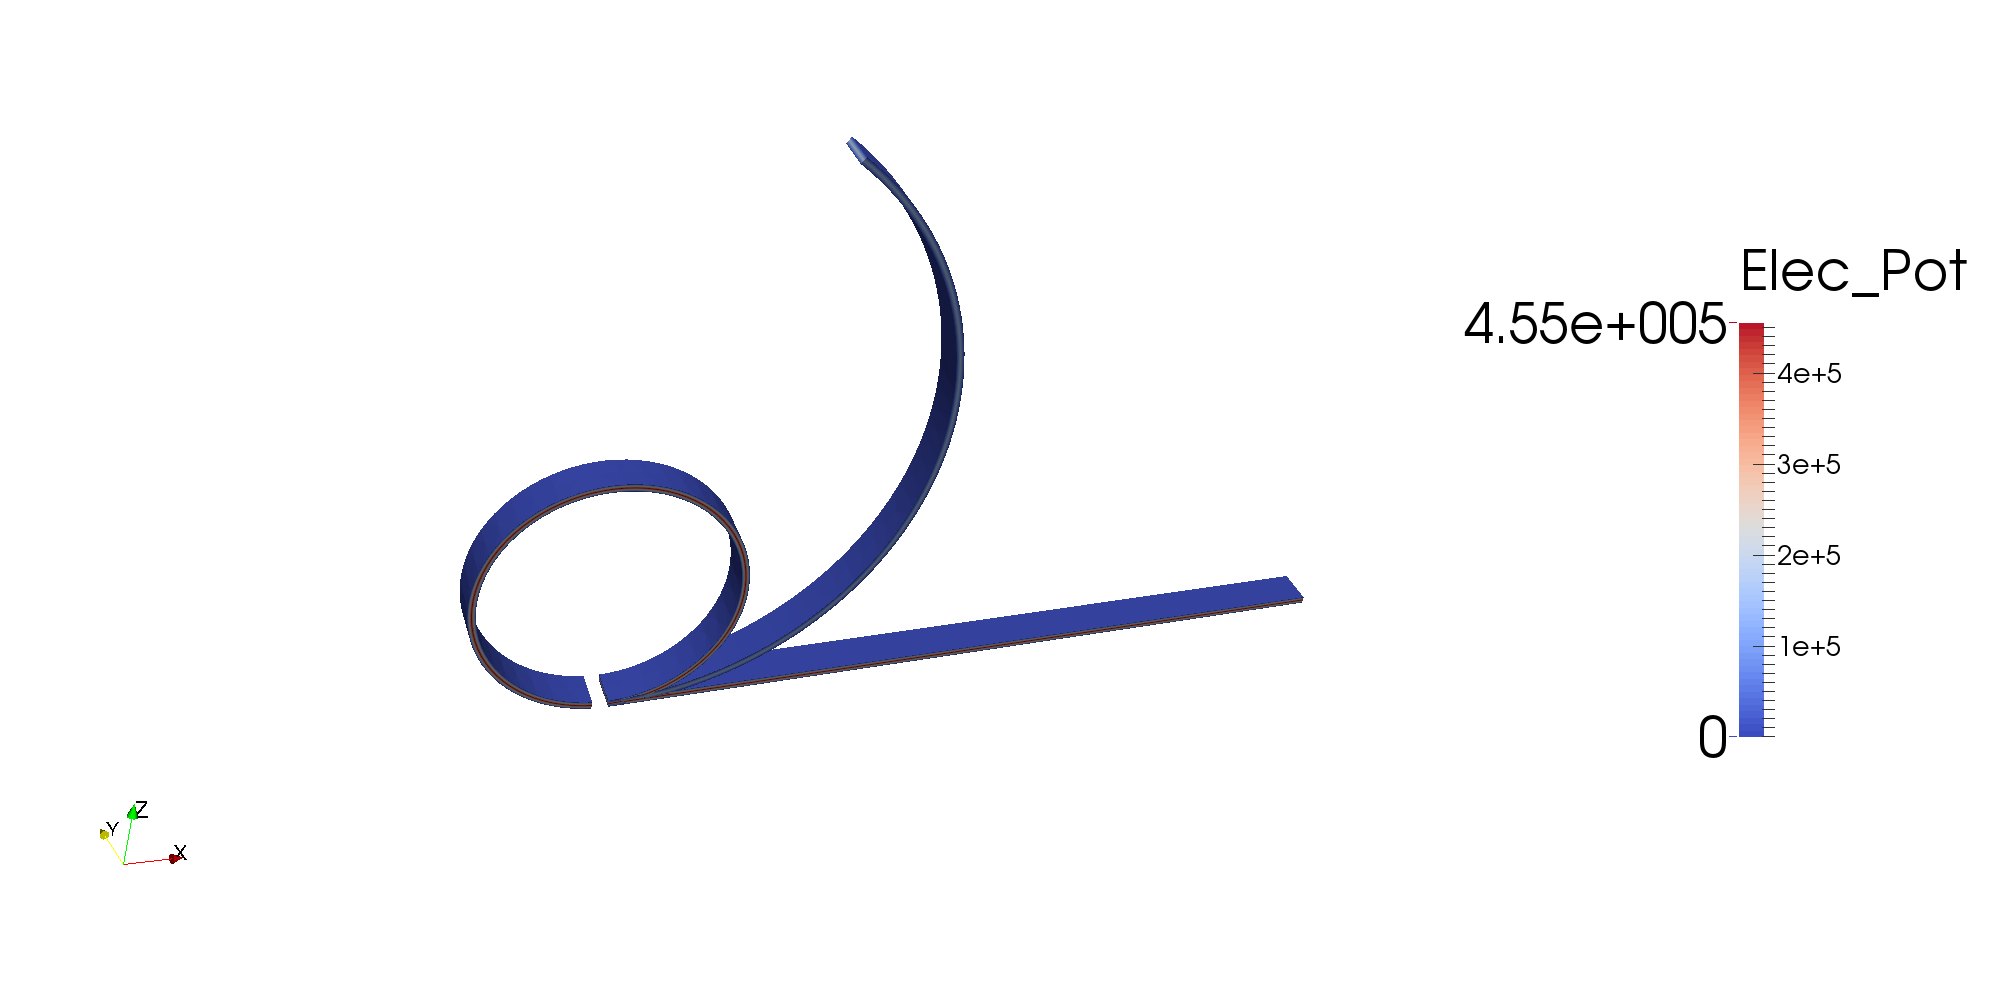
\includegraphics[trim = 00mm 0mm 00mm 0mm,clip=true,width=7.0in]{./chap_4_structural_analyses/pvdf_folding_beam/folding_pvdf_beam.png}
\caption{Folding of bimorph PVDF beam under very high electric potential}
\label{fig:pvdf_beam_folding} 
\end{figure}


\section{Active Fiber Composites}
Active Fiber Composite (AFC) is an actuation architecture that has been introduced to amplify the deflection cased by piezo-electric effect.
The active part is due to PZT5A fibers. 
PZT5A fibers are embedded in the Epoxy matrix and are aligned along the longitudinal direction.
The electric field is applied to PZT5A fiber through the aluminum electrode fingers that are placed on the top and bottom of the fibers.
Aluminum electrode fingers are aligned perpendicular to the longitudinal direction of fiber in the width direction of AFC patch.
Electrodes that are placed on the top and bottom in the thickness direction of the AFC patch have the same electric potential.
Therefore, the electric field on the central plane of the AFC is zero.
Electrodes that are adjacent to each other in the longitudinal direction of the AFC have the opposite electric potentials.
As a result, an electric field is formed in the longitudinal direction of fibers.
The electric field in the gap between electrodes is directly proportional to the valued of applied potential.
The electric field in the gap between electrodes is inversely proportional to the gap distance between electrodes.
An example of AFCs is shown in figure \ref{fig:afc_picture_from_lap}.
Schematic for the placement of fibers and electrodes is shown in \ref{fig:schematic_afc_unit_cell} \cite{jemai2014mathematical}.

\begin{figure} 
\centering
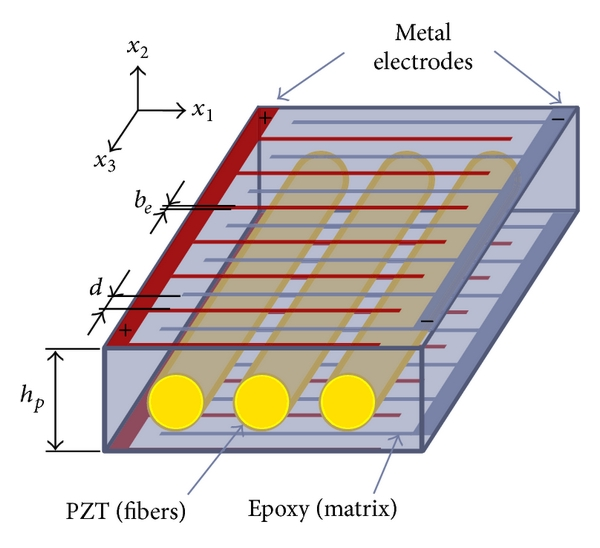
\includegraphics[width=3.0in]{./chap_4_structural_analyses/afc_unit_cell/schematic_afc_unit_cell.jpg}
\caption{Schematic for placement of Fibers and electrodes in the Epoxy matrix \cite{jemai2014mathematical}}
\label{fig:schematic_afc_unit_cell}
\end{figure}

\begin{figure} 
\centering
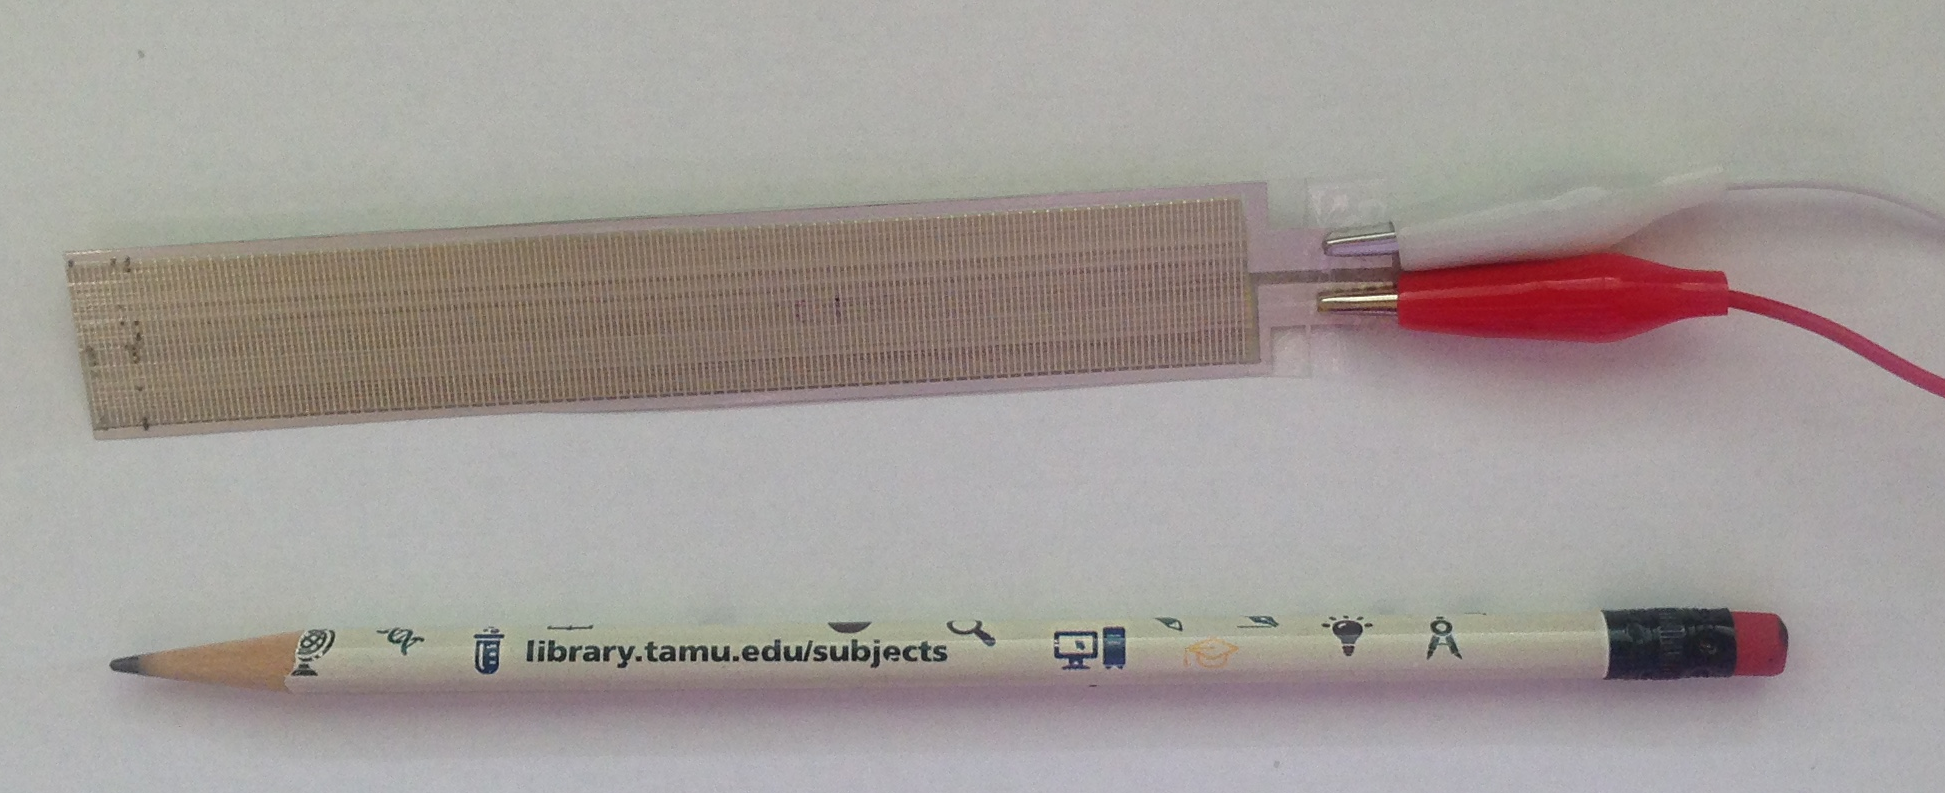
\includegraphics[width=6.0in]{./chap_4_structural_analyses/afc_unit_cell/afc_picture_from_lap.png}
\caption{Active Fiber Composite and applying electric potential}
\label{fig:afc_picture_from_lap}
\end{figure}

The configuration of AFC patch is symmetric with respect to its thickness direction.
Moreover, there is a periodic pattern in the placement of fibers, electrodes and matrix in the longitudinal direction of AFC.
Due to this symmetry and periodic configuration, a unit cell model for AFC is defined as a representative microstructure.
This unit cell can present the overall electro-mechanical behavior of AFC.  
 
\subsection{Unit Cell of an Active Fiber Composite}
The smallest possible unit cell of AFC is considered in order to simulate its overall behavior.
This unit cell contains one quarter of the fiber in the space between two electrodes.
This unit cell of AFC is shown in figure \ref{fig:geometry_unit_cell_afc}.
It is a cubical domain with dimensions of $L_1 \times L_2 \times L_3 =140 \mu m \times 175 \mu m \times 750 \mu m$.
A PZT5A fiber with the radius of $125 \mu m$ is embedded in Epoxy matrix as shown in figure \ref{fig:geometry_unit_cell_afc} (right).
Two Aluminum electrodes can be seen in the unit cell under the fiber with thickness of $10 \mu m$. 
Each Aluminum electrode finger is $250 \mu m$ long due to periodicity of the microstructure only half of each electrode is considered in the unit cell.
There is $500 \mu m$ gap between two electrodes that is filled with Epoxy.
Moreover, there is $4 \mu m$ vertical threshold between the electrodes and PZT5A fiber that is filled with Epoxy.
The electric potential applied to the Aluminum electrodes induces electric field inside the Epoxy and also inside the PZT5A fiber.

\begin{figure} 
\centering
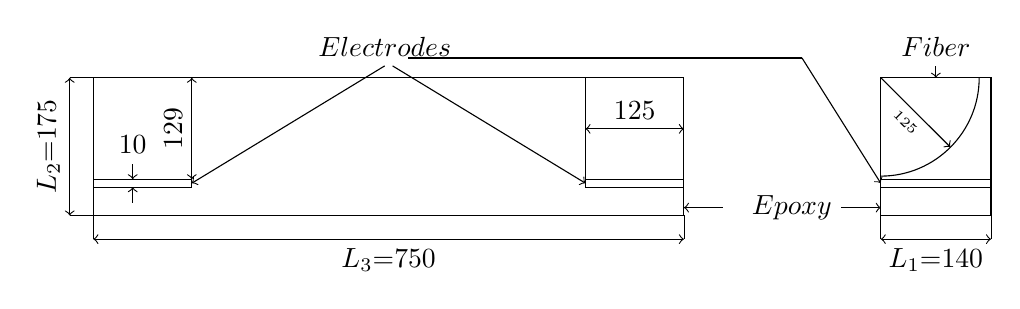
\begin{tikzpicture} 

\draw (0,0) rectangle (7.50,1.75) ; 

\draw (0,0.36) rectangle (1.25,0.46);
\draw (6.25,0.36) rectangle (7.50,0.46); 

 
% dimension in the middle from top to electrode 
\draw [<->] (1.25,0.46) -- (1.25,1.75) node [sloped,midway,above] {129};

% right dimension for  right electrode
\draw  [<-] (0.5,0.46)--(0.5,0.66) node [above] {10};
\draw  [<-] (0.5,0.36)--(0.5,0.16);

%vertical dimenstion
\draw [<->] (-0.30,0) --  (-0.30,1.75) node [sloped,midway,above] {$L_2$=175};
\draw [very thin,-] (0.0,0) --  (-0.30,0);
\draw [very thin,-] (0.0,1.75) --  (-0.30,1.75);

% horizental dimension of electrode
\draw [very thin,-] (6.25,0.36) -- (6.25,1.75);
\draw [<->] (6.25,1.1) --  (7.5,1.1)  node [sloped,midway,above] {125};

%horizentoal dimenstion
\draw [<->] (0,-0.30) --  (7.50,-0.30) node [sloped,midway,below] {$L_3$=750};
\draw [very thin,-] (0,0) --  (0,-0.30);
\draw [very thin,-] (7.5,0) --  (7.5,-0.30);

%% The left view
\draw (10.0,0) rectangle (11.4,1.75) ; 
%% The horizental dimension
\draw [<->] (10.0,-0.3)--  (11.4,-0.3) node [sloped,midway,below] {$L_1$=140};
\draw [very thin,-] (10.0,0) --  (10.0,-0.3);
\draw [very thin,-] (11.4,0) --  (11.4,-0.3);

%% The fiber
\draw (11.25,1.75) arc  (0:-90:1.25) ; 
%% The electode in the view
\draw (10.0,0.36) rectangle (11.4,0.46) ;

%% The arrows for electrodes
\draw [<-] (1.25,0.41) -- (3.7,1.9) node [above] {$Electrodes$};
\draw [<-] (6.25,0.41) -- (3.8,1.9) ;
\draw [<-] (10.0,0.41) -- (9,2.0) ;
\draw (9,2.0) -- (4.00,2.0) ;

%% The arrows for fiber
\draw [<-] (10.7,1.75) -- (10.7,1.9) node [above] {$Fiber$};

%% The arrows for Epoxy
\draw [<-] (10.0,0.10) -- (9.5,0.1) node [left] {$Epoxy$};
\draw [<-] (7.50,0.10) -- (8.0,0.1);

%% The radial dimension
\draw [<-] (10.883,0.8698) -- (10.0,1.75)  node [sloped,midway,below]{\tiny 125};

\end{tikzpicture}
\caption{Geometry of Unit Cell (dimensions are in $\mu m$)}
\label{fig:geometry_unit_cell_afc}
\end{figure}

The mechanical response of Epoxy is considered to be linear visco-elastic.
The Epoxy is assumed to have very small electro-mechanical coupling that can be excluded from the analyses.
The electric potential is transferred from the electrodes to fibers through the Epoxy.
Therefore, the dielectric properties of Epoxy has significant effect on overall electro-mechanical properties of AFC \cite{atitallah2014parametric}. 
The electric potential are applied to the two aluminum electrodes which, are shown in the unit cell in the figure \ref{fig:geometry_unit_cell_afc}.
The embedded aluminum electrodes have $10 \mu m$ thickness.
It is noted that only half of each electrode is considered in this unit cell.
The length of each electrode is $250 \mu m$.
Two electrodes that are considered in the unit cell are charged with electric potential with an opposite sign.
The response of Aluminum on the AFC is assumed to be linear a elastic.

The periodic and symmetric boundary conditions are applied to the unit cell in order to model the effective behavior of AFC. 
The boundary conditions prescribe on the unit cell of AFC are given as follows:

\begin{equation}
\begin{aligned} 
& x_1=-\frac{L_1}{2}  ,& u_1=0 &\, , \frac{\partial \phi}{\partial x_1}=0        &\, ; \ x_1= \frac{L_1}{2}  ,& u_1=\bar{u_1} &\, ,  \frac{\partial \phi}{\partial x_1}=0   \\ 
& x_2=-\frac{L_2}{2}  ,& u_2=0 &\, , \frac{\partial \phi}{\partial x_2}=0        &\, ; \ x_2= \frac{L_2}{2}  ,& u_2=\bar{u_2} &\, ,  \frac{\partial \phi}{\partial x_2}=0   \\ 
& x_2=-\frac{L_3}{2}  ,& u_2=0 &\, , \frac{\partial \phi}{\partial x_3}=0        &\, ; \ x_3= \frac{L_3}{2}  ,& u_3=\bar{u_3} &\, , \frac{\partial \phi}{\partial x_3}=0    \\
\end{aligned}
\end{equation}
where the geometry of the unit cell is defined in $x_1 \in [-L_1/2,L_1/2], x_2 \in [-L_2/2,L_2/2], x_3 \in [-L_3/2,L_3/2]$.


The matrix, electrodes and fibers are glued together.
It is assumed that the glue has the same mechanical and electrical properties as the Epoxy.
Only the piezoelectric fiber experiences electro-mechanical coupling due to the applied electric field.
The strain induced inside the fiber causes deformations of the unit cell.
The visco elastic properties of the Epoxy and the time
 dependent electro-mechanical response of piezo electric fiber can affect the overall deflection of the unit cell.
The finite element analyses for nonlinear time-dependent electro-mechanical response are used to simulate and predict the behavior of AFC. 

The electric potential is applied to the electrodes in the unit cell.
The material properties that are taken for PZT5A fiber, Epoxy matrix and aluminum electrodes are presented in table \ref{table:materila_properties_afc}.
% It is assumed that electro-mechanical response of PZT5A fiber is time dependent.
% In addition, visco-elastic behavior of Epoxy matrix is considered in this analyses.
% The Aluminum electrodes are considered elastic with no time dependent behavior.
% The electric potential is uniform inside the metallic electrodes. The electric potential should pass through the matrix to reach the PZT5A fiber.
% This makes the dielectric properties of matrix an important factor in the overall electro-mechanical property of AFC patch \cite{atitallah2014parametric}. 
The distribution of electric potential is shown in figure \ref{fig:electrip_potential_afc_pictur}.
In this picture the positive and negative electric potentials applied to the unit cell are shown.

\begin{table}
\caption{Material Properties of AFC}
\centering
\begin{tabular}{|l|c|c|c|r|}
\hline
               & PZT5A & Epoxy & Aluminum & \\ \hline 
Young's Modulus&60.06 & 1.5     & 69       &$GPa$    \\ \hline
Poisson's Ratio&$0.3$ & 0.35    & 0.33 &\\ \hline 
$e_{113}$      &-59.5 &         &      &$C/m^2$\\ \hline
$e_{311}$      &8.00&         &      &$C/m^2$\\ \hline
$e_{333}$      &-27.196  &         &      &$C/m^2$\\ \hline
$\kappa_{11}=\kappa_{22}$ &  $ 4  $ & $8.854  $ & &  pF/m \\ \hline
$\kappa_{33}$ & $2  $              & $8.854  $ & &  pF/m \\ \hline
${}^{0}K_{ijk}^{e}$&1.0& & &  \\ \hline
${}^{1}K_{ijk}^{e}$&-0.45& & & \\ \hline
${}^{0}\lambda_{ijk}^{e}$&0& & & s \\ \hline
${}^{1}\lambda_{ijk}^{e}$&1.5& & & s \\ \hline 
${}^{0}K_{ijkl}^{c}$& &1.0 & &  \\ \hline 
${}^{1}K_{ijkl}^{c}$& &0.4 & & \\ \hline
${}^{0}\lambda_{ijkl}^{c}$& &0&  & s\\ \hline
${}^{1}\lambda_{ijkl}^{c}$& &0.8 & & s \\ \hline 
\end{tabular}
\label{table:materila_properties_afc} 
\end{table}

\begin{figure} 
\centering
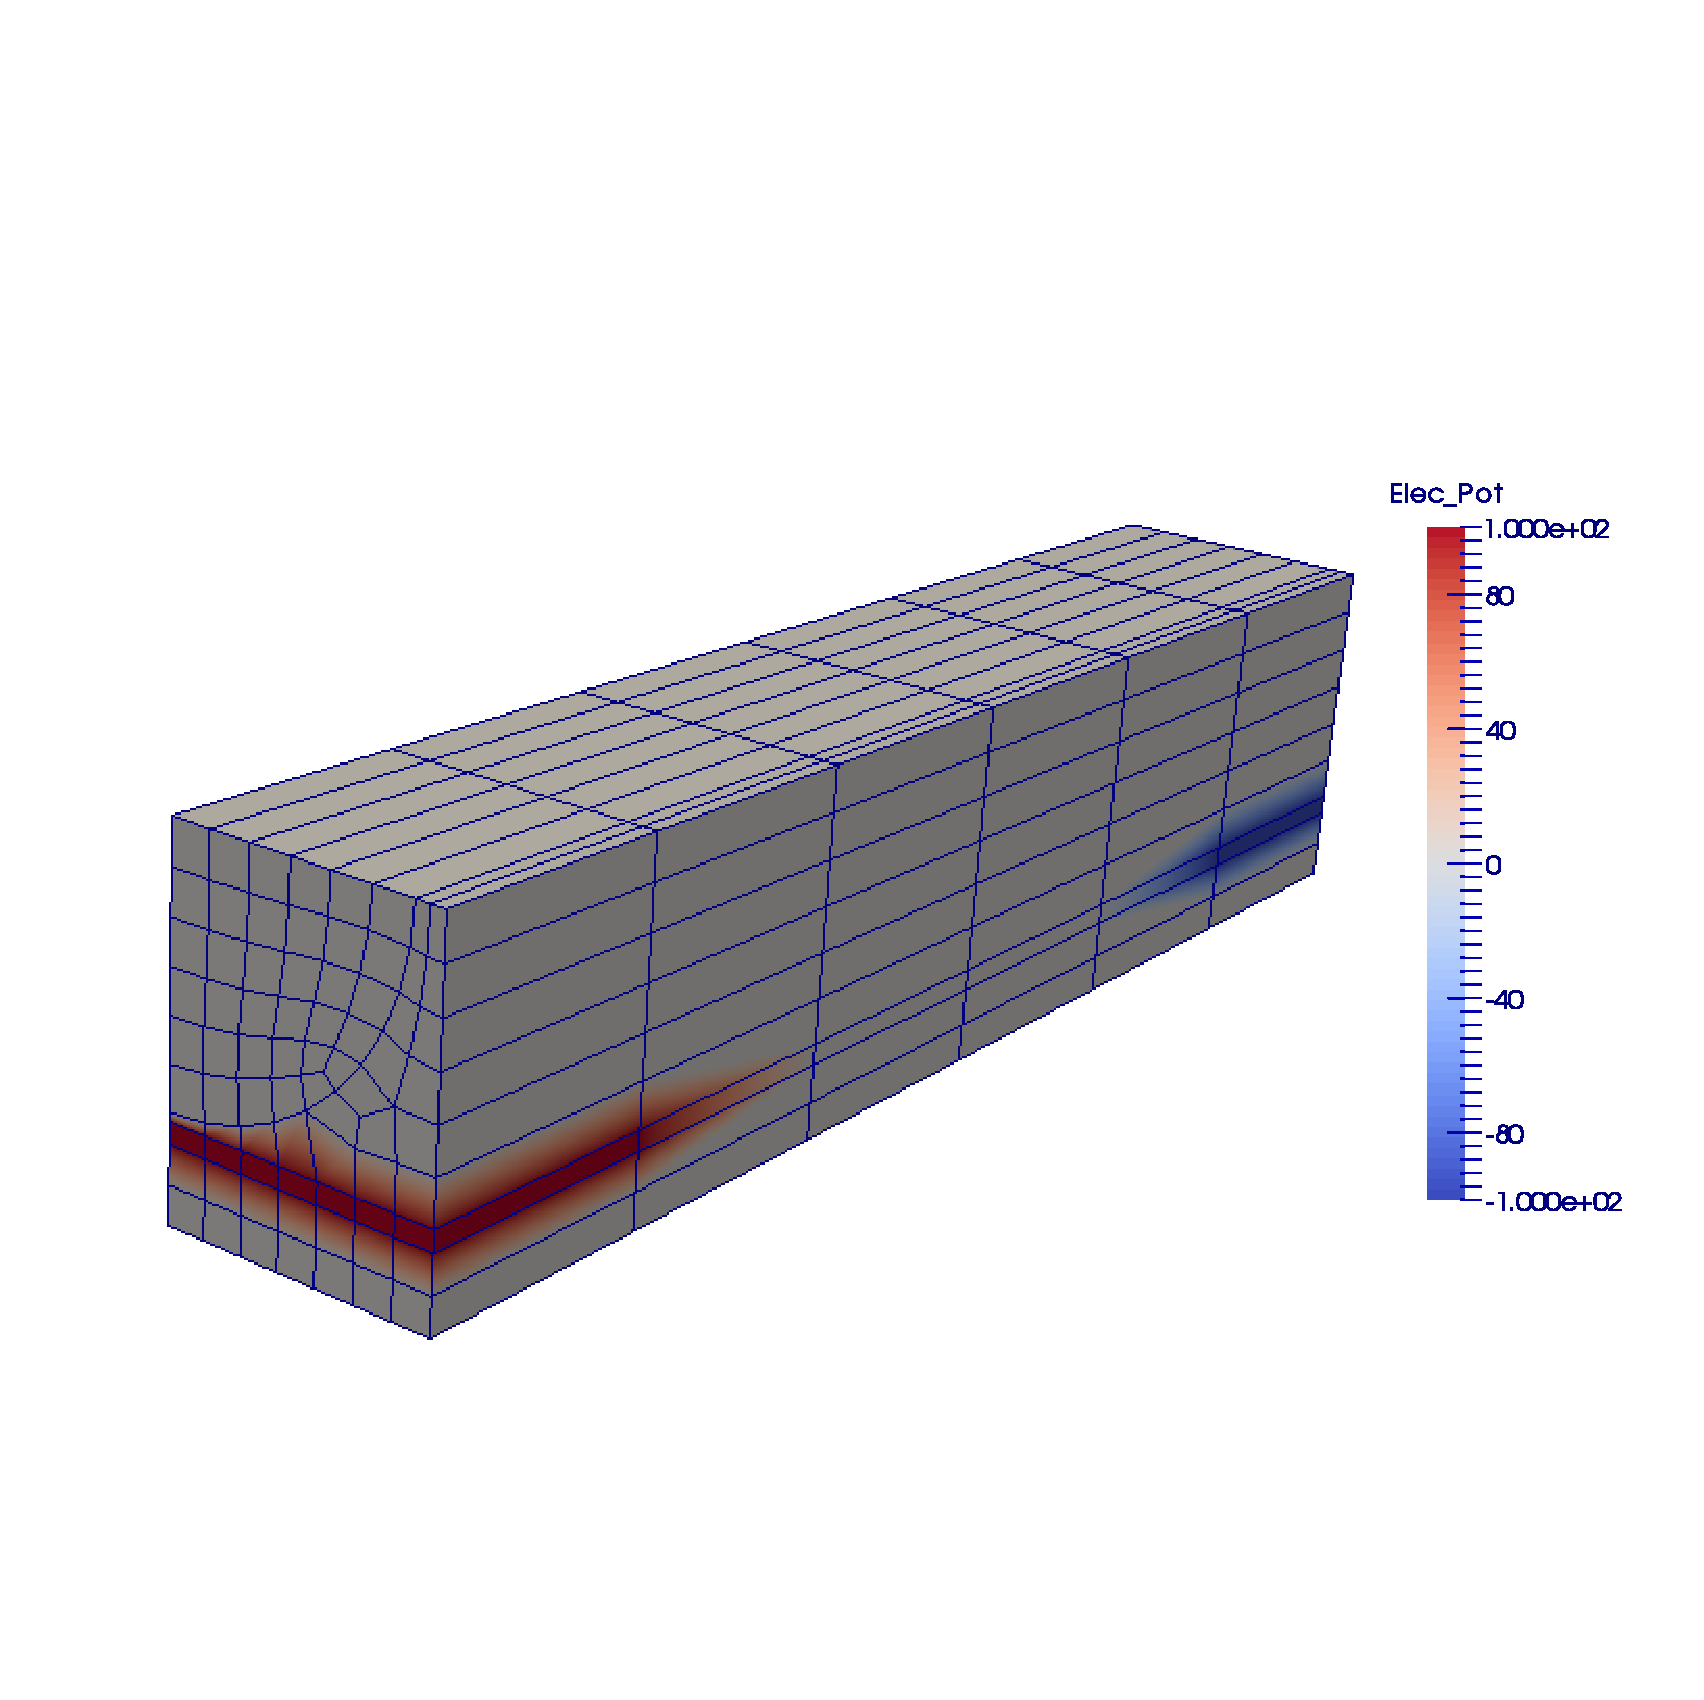
\includegraphics[width=3.0in]{./chap_4_structural_analyses/afc_unit_cell/afc_electrip_petential_distribution.pdf}
\caption{Active Fiber Composite distribution of electric potential in its unit cell}
\label{fig:electrip_potential_afc_pictur}  
\end{figure}  

\begin{figure} 
\centering
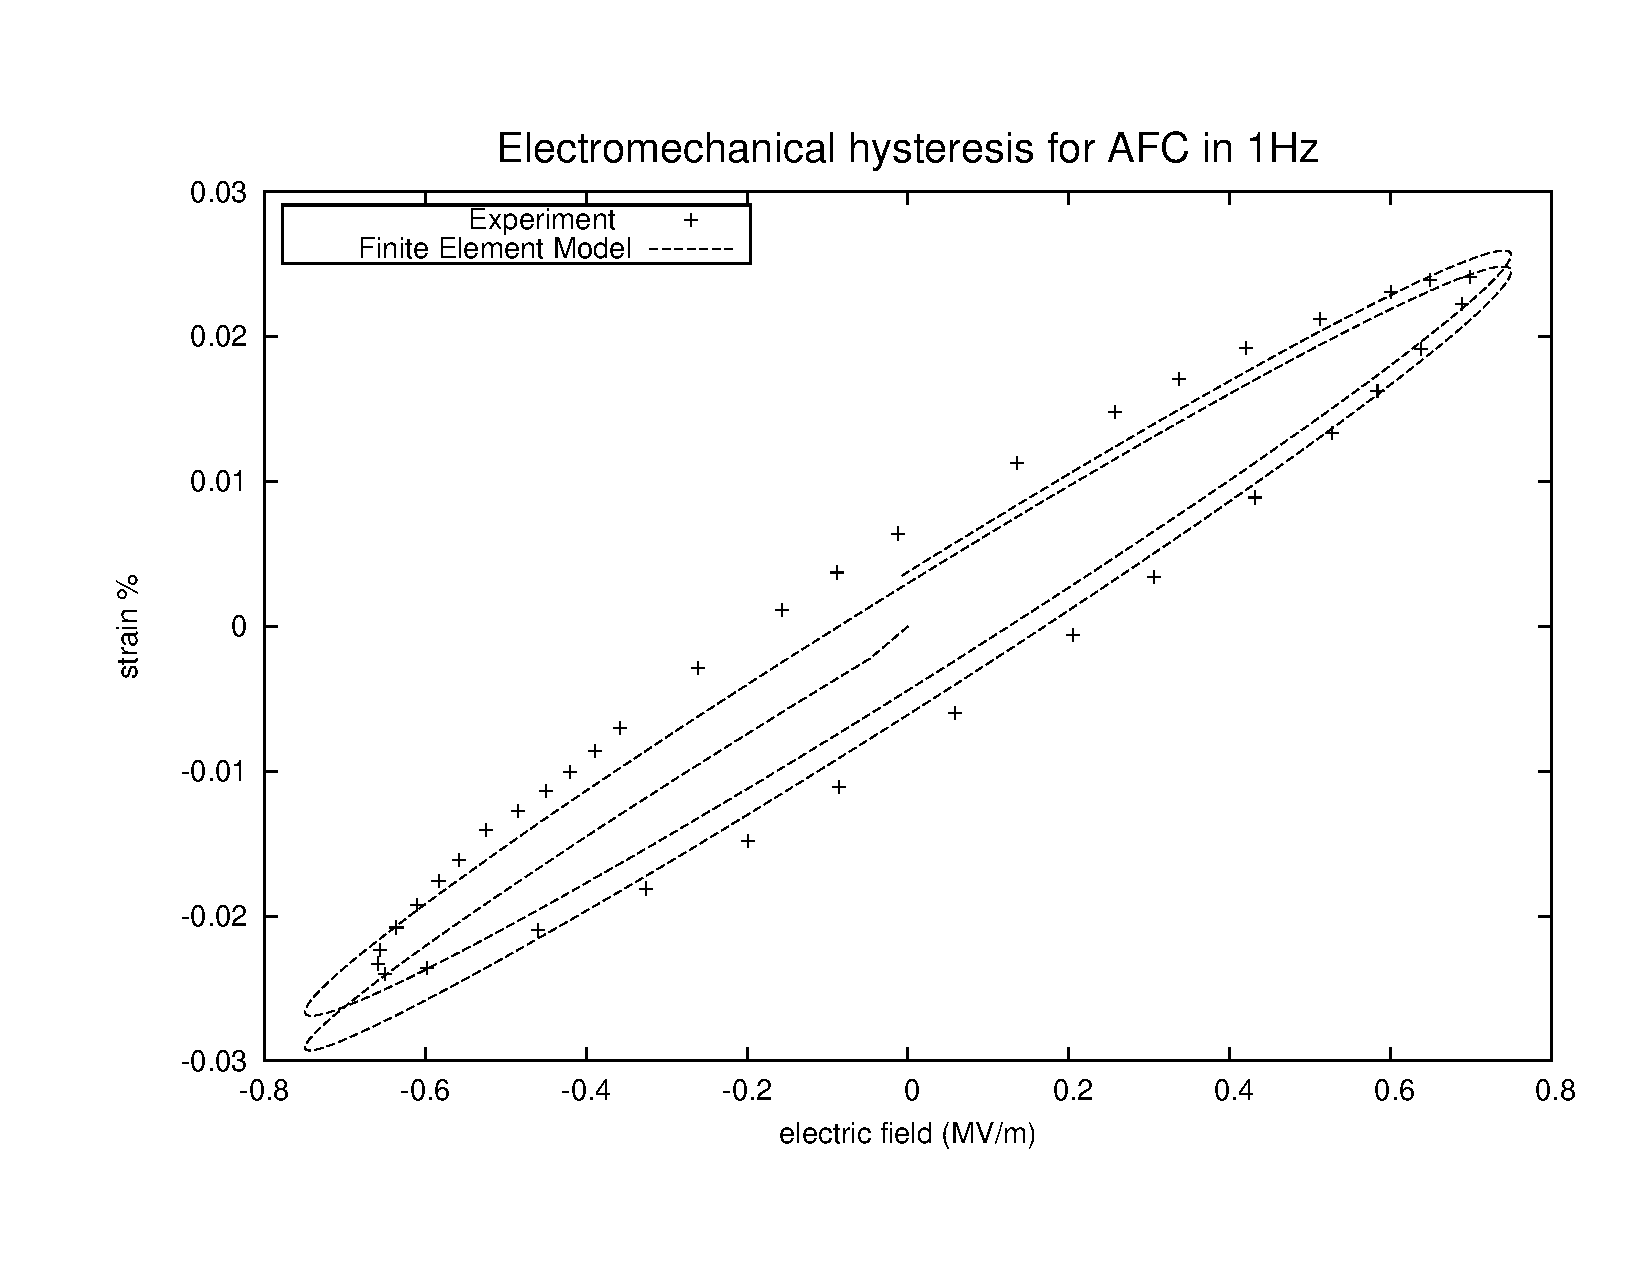
\includegraphics[width=5.0in]{./chap_4_structural_analyses/afc_unit_cell/comparison/afc_result_electric_field_vs_strain.pdf}
\caption{Electro-mechanical hysteresis at 1Hz compared with experiment}
\label{fig:afc_result_electric_field_vs_strain}
\end{figure} 

\subsection{Validating The AFC Model with Experiment Data}
The finite element analyses for AFC unit cell is validated with the existing experimental results.
The detailed experimental procedure is discussed in [On the temperature and time dependence of the electro-mechanical properties flexible active fiber composites].
In order to calibrate the properties of PZT, line between two peaks of the hysteresis curve from experimental data is used to find the linear and time independent material properties.
The material properties Epoxy and Aluminum are taken from \cite{atitallah2014parametric}.
The Aluminum as considered elastic and its material property is taken from \cite{Aluminium_wikipedia}.
Then, the width of hysteresis curve is used as a reference to choose the Proney series coefficient presented in table \ref{table:materila_properties_afc}.
 
The comparison between experimental results and results from finite element analyses with linear time dependent electro-mechanical coupling for PZT is shown in figure \ref{fig:afc_result_electric_field_vs_strain}.
The hysteresis response shown in the deflection of this unit cell is due to the time dependent response of the Epoxy matrix and also time dependent electro-mechanical coupling of piezo-electric fiber. 
There is good comparison between the experiments and finite element analyses.
The distribution of displacement field in the unit cell is shown in figure \ref{afc_displacement_all:fig}.
As it is expected the value of displacement in longitudinal (displacement Z) is significantly larger than the other two directions.

\begin{figure} 
\centering
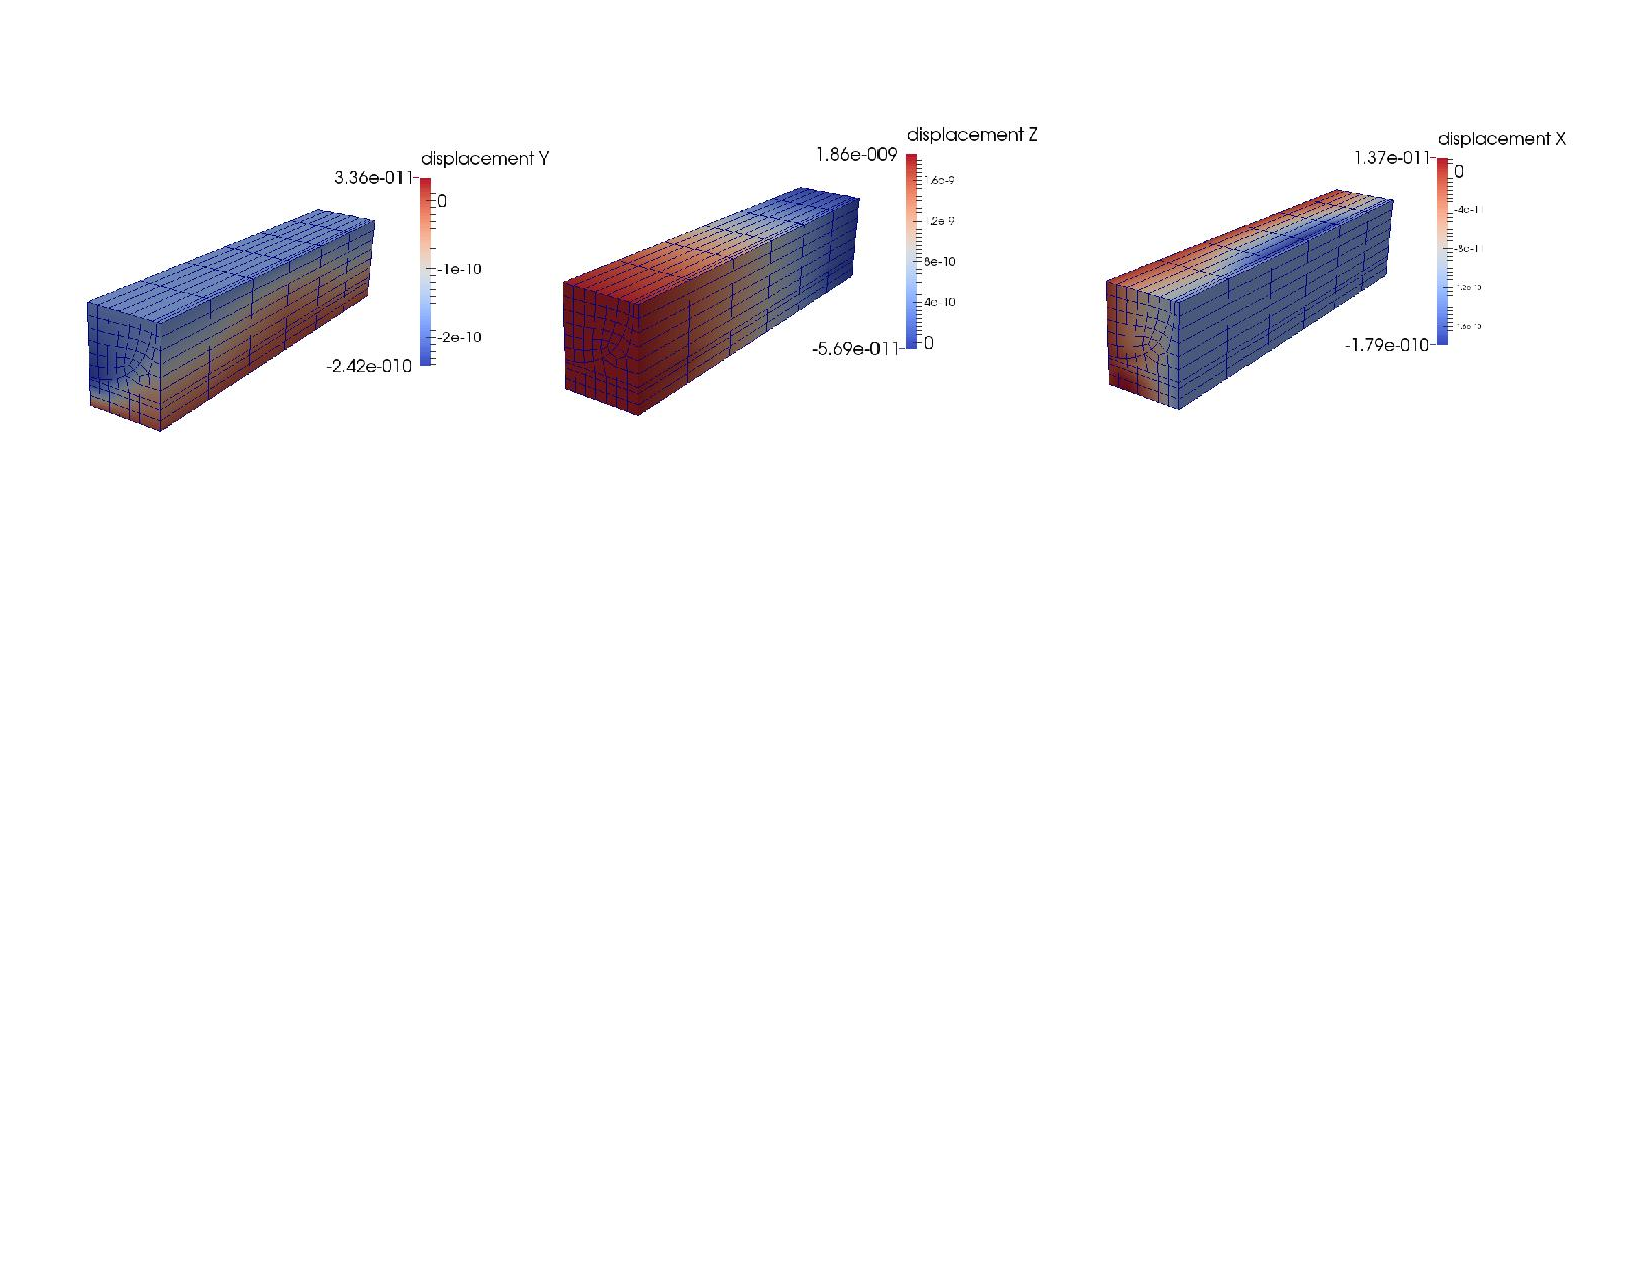
\includegraphics[trim = 0mm 100mm 0mm 0mm,width=6.0in]{./chap_4_structural_analyses/afc_unit_cell/afc_displacement_all.pdf}
\caption{Displacement field distribution in unite cell of AFC in mm}
\label{afc_displacement_all:fig}
\end{figure}

At higher amplitudes of electric field AFC shows nonlinear and time dependent response due to nonlinear electromechanical coupling. 
This effect is simulated using the QLV model that has been disuses in the previous chapters. 
A polynomial for the nonlinear electric field is considered. The material parameters for this model are presented in Table \ref{table:non_linear_materila_properties_afc}.
It can be seen that model is in good agreement with the experimental results.
The deviation between the result from experiment and numerical results in higher amplitude of electric field could be due to effect of polarization switching in some parts of piezoelectric fiber.
It is noted that in the AFC and distribution of electric potential inside the fiber is not uniform.
In some part of fiber where the intensity of electric field is larger than the coercive field, there is a change in polarization of PZT.
This effect will cause large deviation between the result from the current analyses for minor effect.


\begin{table}
\caption{Nonlinear Material Properties of AFC}
\centering
\begin{tabular}{|l|c|c|c|r|}
\hline
               & PZT5A & Epoxy & Aluminum & \\ \hline 
Young's Modulus&60.06 & 1.5     & 69       &$GPa$    \\ \hline
Poisson's Ratio&$0.3$ & 0.35    & 0.33 &\\ \hline 
$e_{113}$      &-18.9 &         &      &$C/m^2$\\ \hline
$e_{311}$      &9.82&         &      &$C/m^2$\\ \hline
$e_{333}$      &-8.0  &         &      &$C/m^2$\\ \hline
$\kappa_{11}=\kappa_{22}$ &  $ 4  $ & $8.854  $ & &  pF/m \\ \hline
$\kappa_{33}$ & $2  $              & $8.854  $ & &  pF/m \\ \hline
${}^{0}K_{ijk}^{e}$&1.0& & &  \\ \hline
${}^{1}K_{ijk}^{e}$&-0.6& & & \\ \hline
${}^{0}\lambda_{ijk}^{e}$&0& & & s \\ \hline
${}^{1}\lambda_{ijk}^{e}$&1.5& & & s \\ \hline 
${}^{0}K_{ijkl}^{c}$& &1.0 & &  \\ \hline
${}^{1}K_{ijkl}^{c}$& &0.1 & & \\ \hline
${}^{0}\lambda_{ijkl}^{c}$& &0&  & s\\ \hline
${}^{1}\lambda_{ijkl}^{c}$& &0.8 & & s \\ \hline 
$\widehat{b}_{3333}$ & $1.5 \times 10^{-5}$ &  $ N/V^2 $\\ \hline
\end{tabular}
\label{table:non_linear_materila_properties_afc} 
\end{table} 
 
\begin{figure} 
\centering
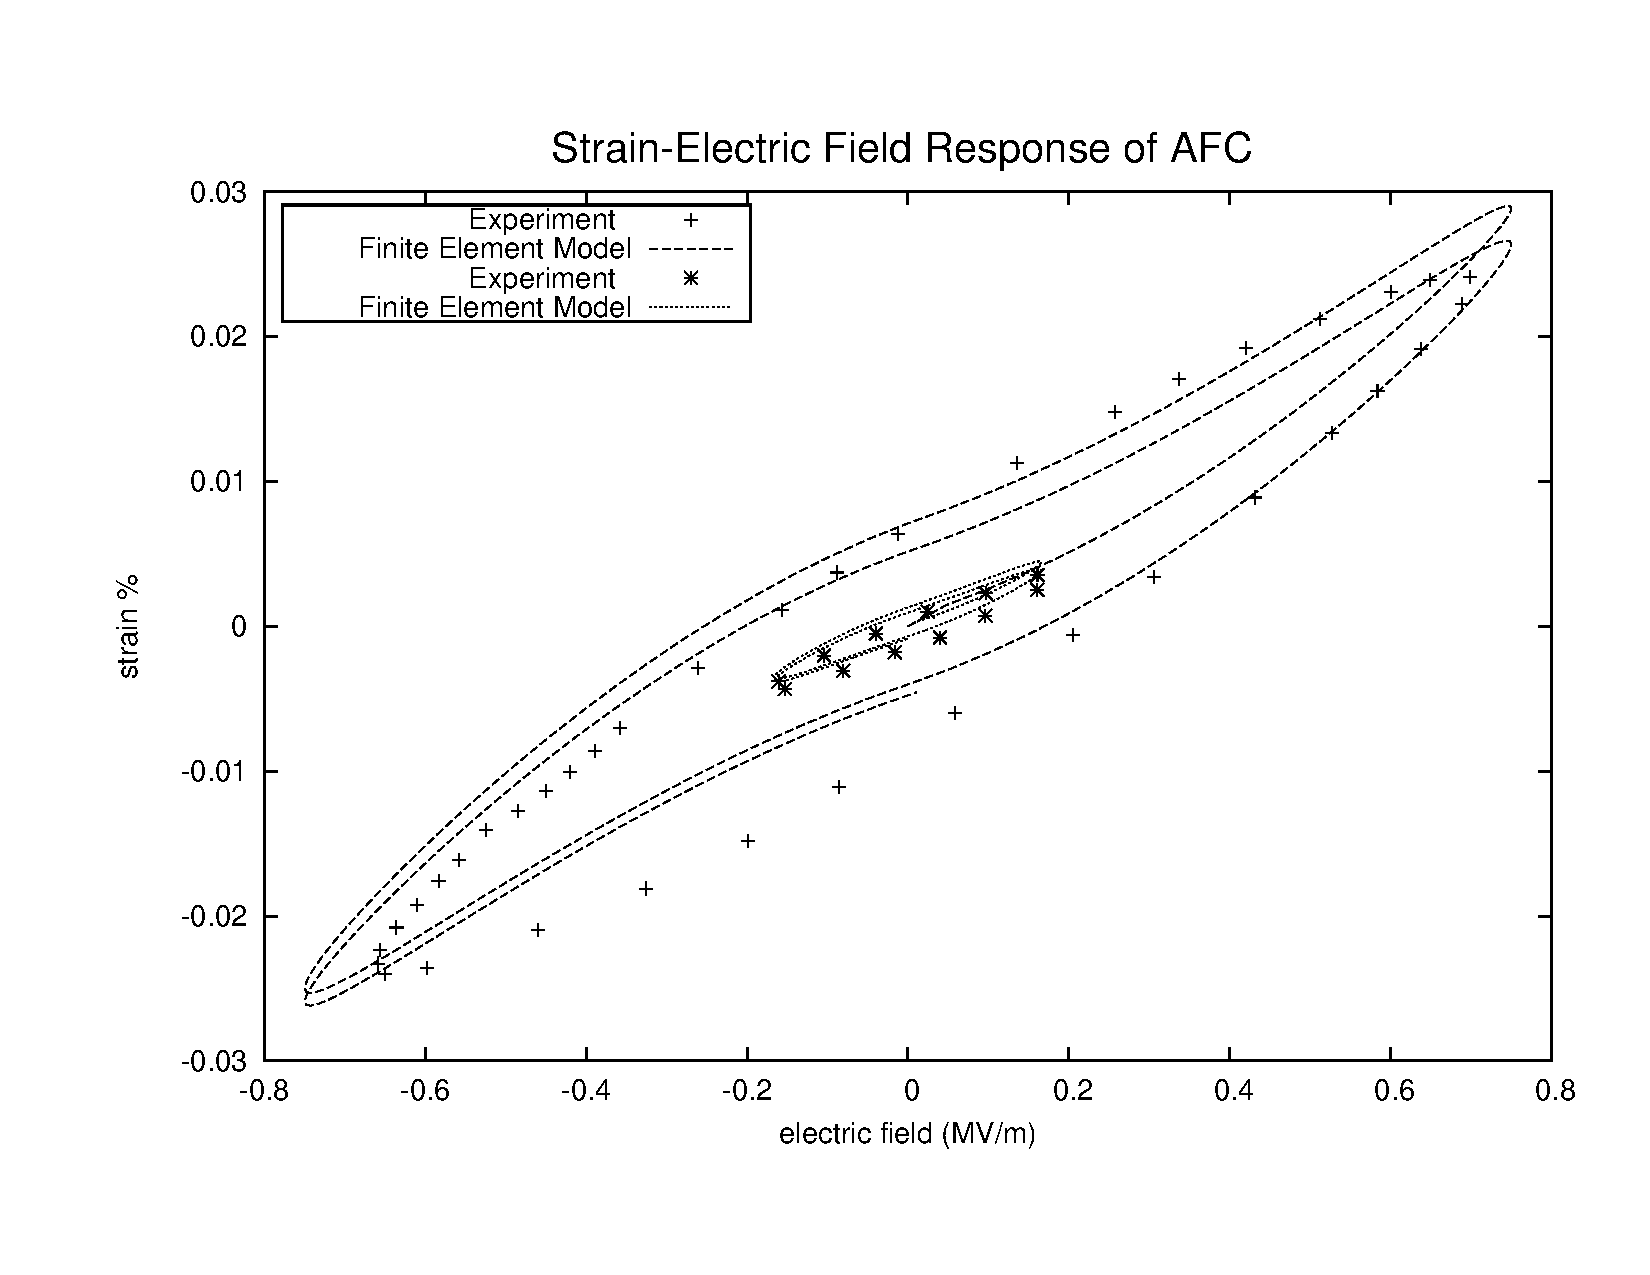
\includegraphics[trim = 0mm 0mm 0mm 0mm,width=5.0in]
{./chap_4_structural_analyses/afc_unit_cell/non_linear_hysteris_afc/non_linear_electric_field_vs_polarization.pdf}
\caption{Nonlinear electro-mechanical hysteresis for different electric fields at 1Hz compared with experiment}
\label{fig:non_linear_electric_field_vs_polarization}
\end{figure}

\subsection{The effect of scale time on electro mechanical response of AFC}
It can be shown that at higher intensity of electric field the piezoelectric materials respond faster to the change in electric field.
We use the same analogy with thermorheologically simple materials that have widely used for mechanical response of polymers \cite{haj2004numerical, tscharnuter2012nonlinear}.
The time scale factor is defined as an exponential function with respect to the electric field intensity $|\textbf {E}|$.
Then the 



\begin{equation}
	\Delta t _{scaled} = \frac{ \Delta t } { a_{ |\textbf {E}| } ) }
\label{equation:time_scaling}	
\end{equation}

where ${a(|\textbf {E}|)}$ is the time shift factor that is defined with respect to norm of electric field vector and a material constant.
 
\begin{equation}
a_{ |\textbf {E}| }=e^{-\gamma_{E} \times |\textbf {E}|}
\label{equation:time_scaling_factor}	
\end{equation}
 
\begin{figure} 
\centering
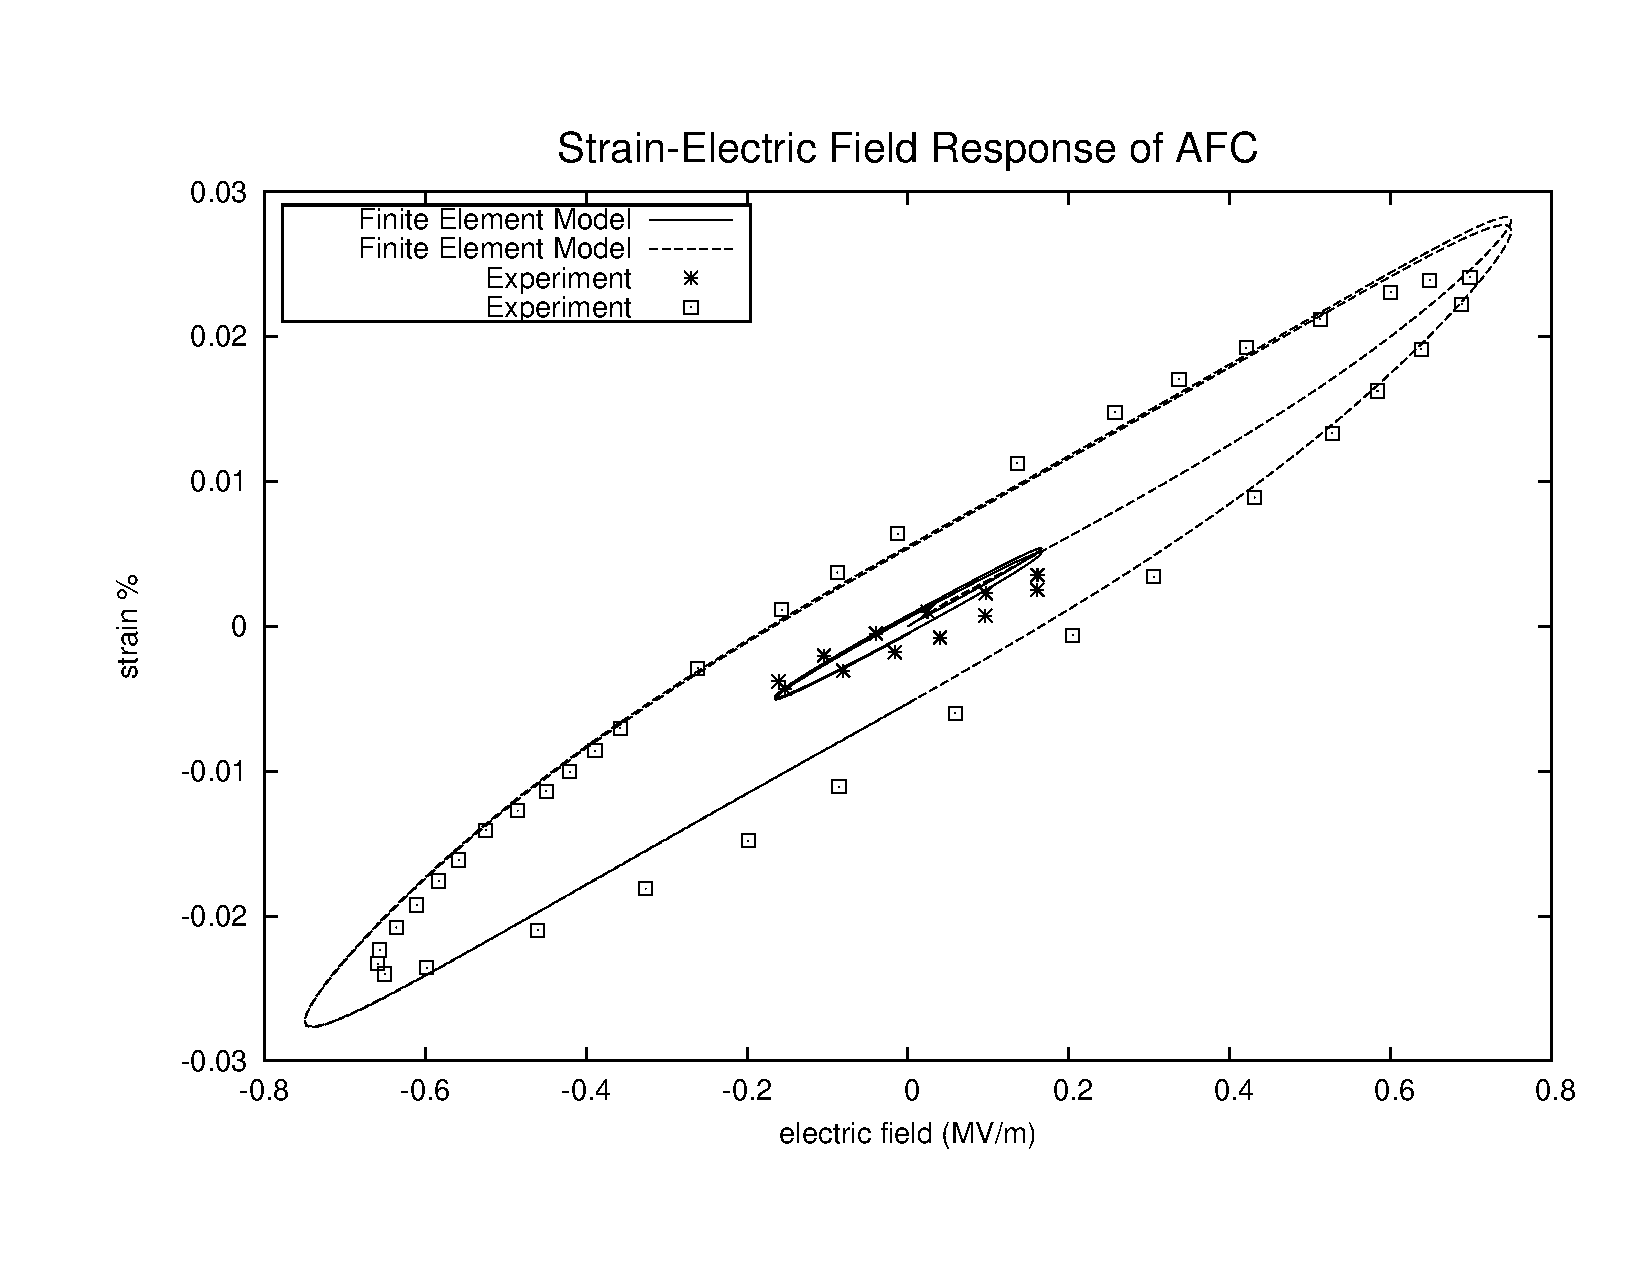
\includegraphics[trim = 0mm 0mm 0mm 0mm,width=5.0in]
{./chap_4_structural_analyses/afc_unit_cell/linear_hysteris_time_shift_afc/time_shift_afc_electric_field_vs_strains.pdf}
\caption{Linear electro-mechanical hysteresis response of AFC model with time shift for different electric fields at 1Hz compared with experiment}
\label{fig:time_shift_afc_electric_field_vs_strains}
\end{figure}

Figure \ref{fig:time_shift_afc_electric_field_vs_strains} shows the result of linear analyses, including the time shift concept for piezoelectric materials.
The time shift material constant is taken as $\gamma_{E}=1.75 m/MV$ for this analyses.

In order to examine the rate (frequency) dependent response, parametric studies are presented by applying electric fields at various frequencies. 
Different frequency inputs are applied to the same material constitutive model presented in this section. 

The corresponding strains response of the model under different frequencies and amplitudes are shown in Figure \ref{fig:afc_Frequency_Effect}. 
It is apparent from the results that higher frequency of loading reduces time-dependent (hysteresis) effect. 
This is due to the fact that the material does not have enough time to exhibit time-dependent effect. 
Fast loading reduces the creep-like or relaxation-like behavior and the area inside the hysteresis curve becomes smaller. 
Even for small frequencies of applied electric field the response of AFC is faster in higher electric field. 
This is due to inclusion of time shift in the model. 
This is the main reason for the pointy shape of hysteresis curves in smaller frequencies. 

\begin{figure}
\centering
\subcaptionbox{Frequency 0.1 Hz}
{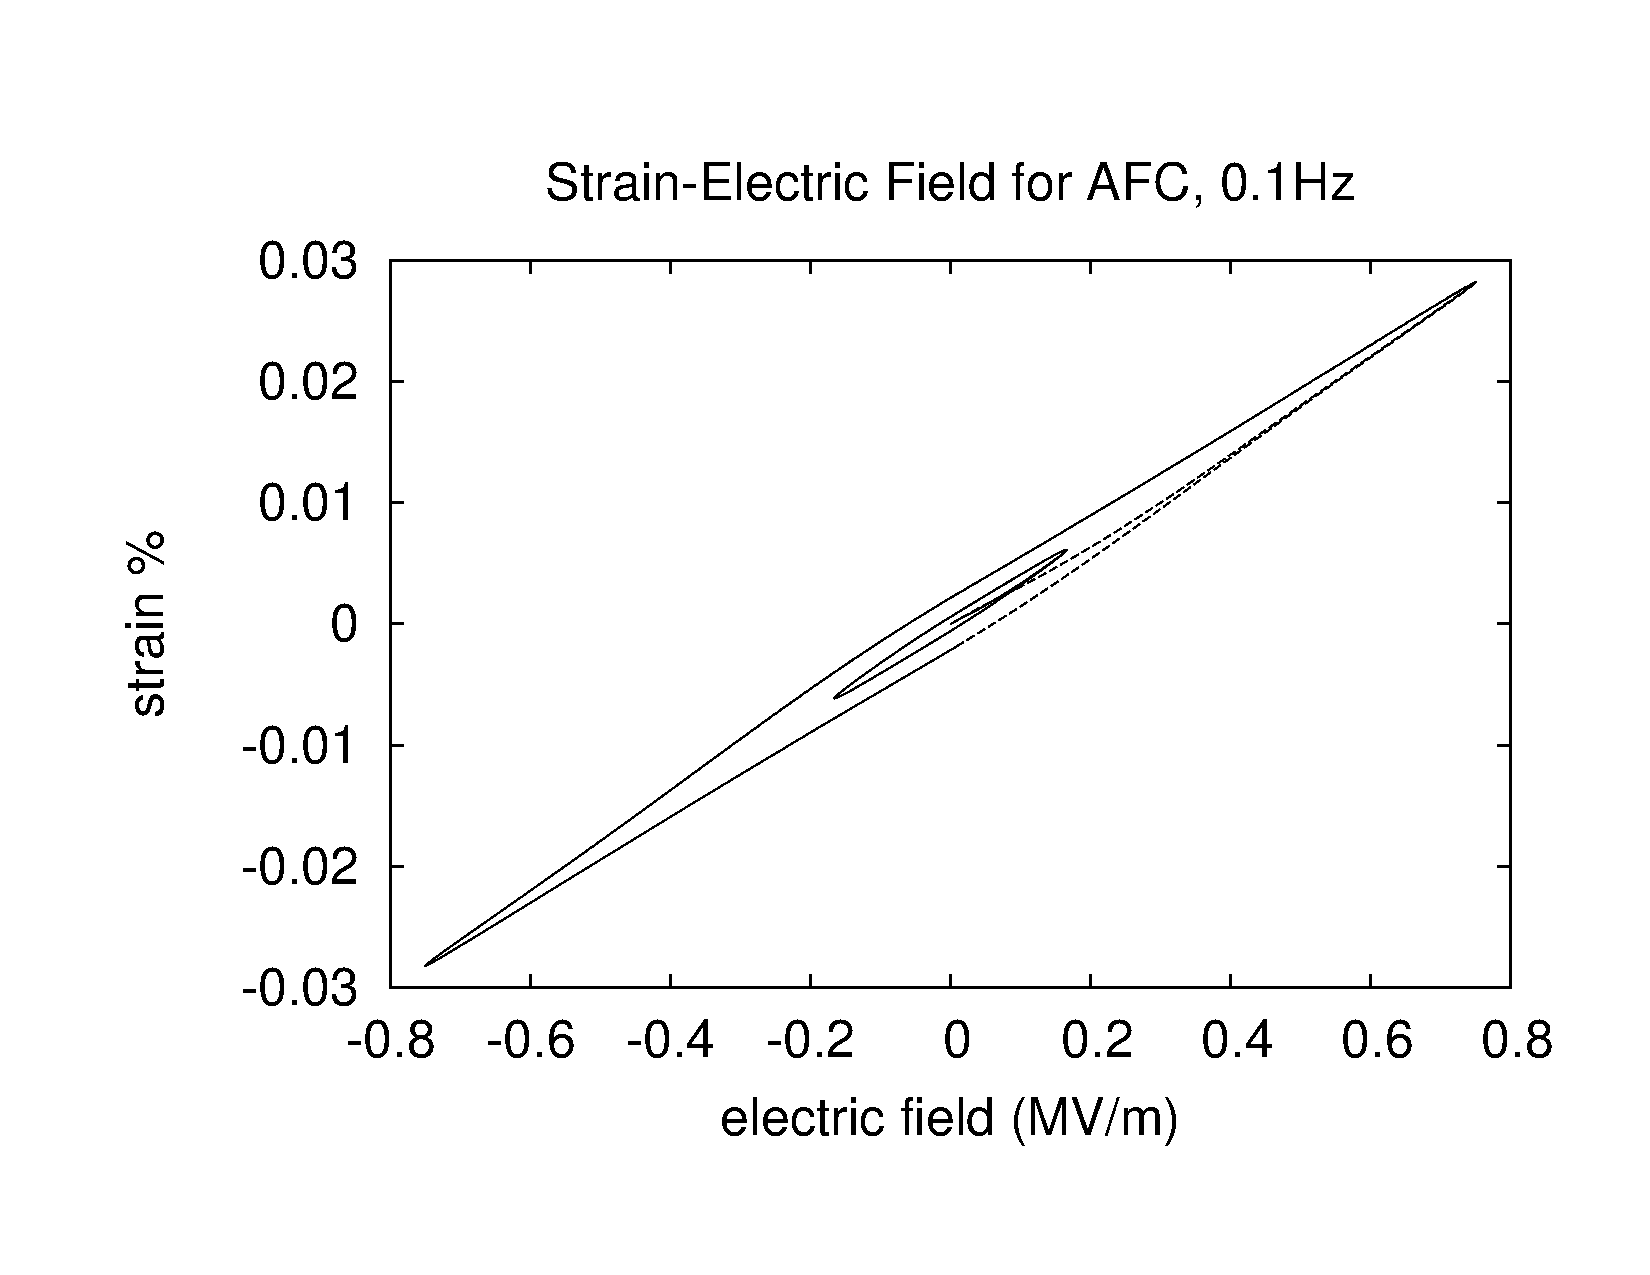
\includegraphics[width=2.5in]{./chap_4_structural_analyses/afc_unit_cell/frequency_effect/electric_field_vs_strains_freq_0p1}}
\subcaptionbox{Frequency 0.2 Hz}
{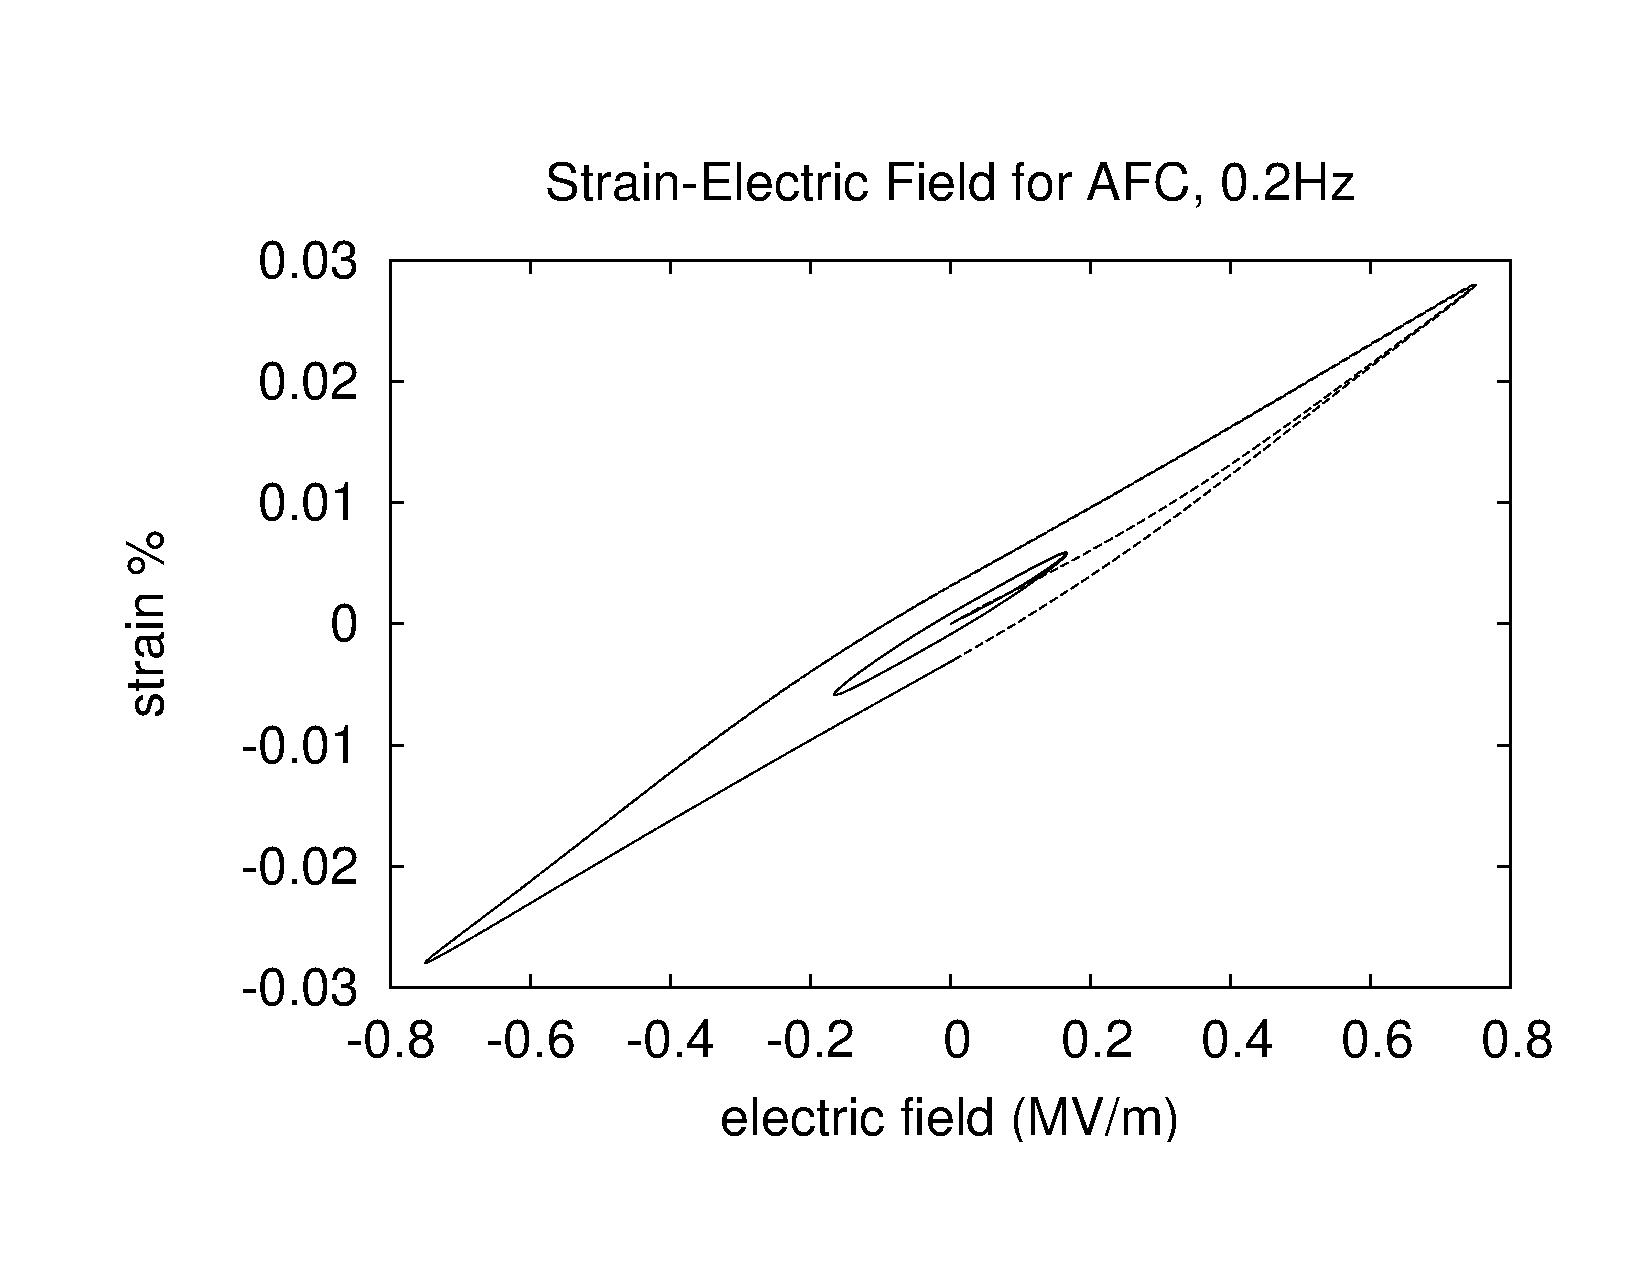
\includegraphics[width=2.5in]{./chap_4_structural_analyses/afc_unit_cell/frequency_effect/electric_field_vs_strains_freq_0p2}}
\subcaptionbox{Frequency 0.5 Hz}
{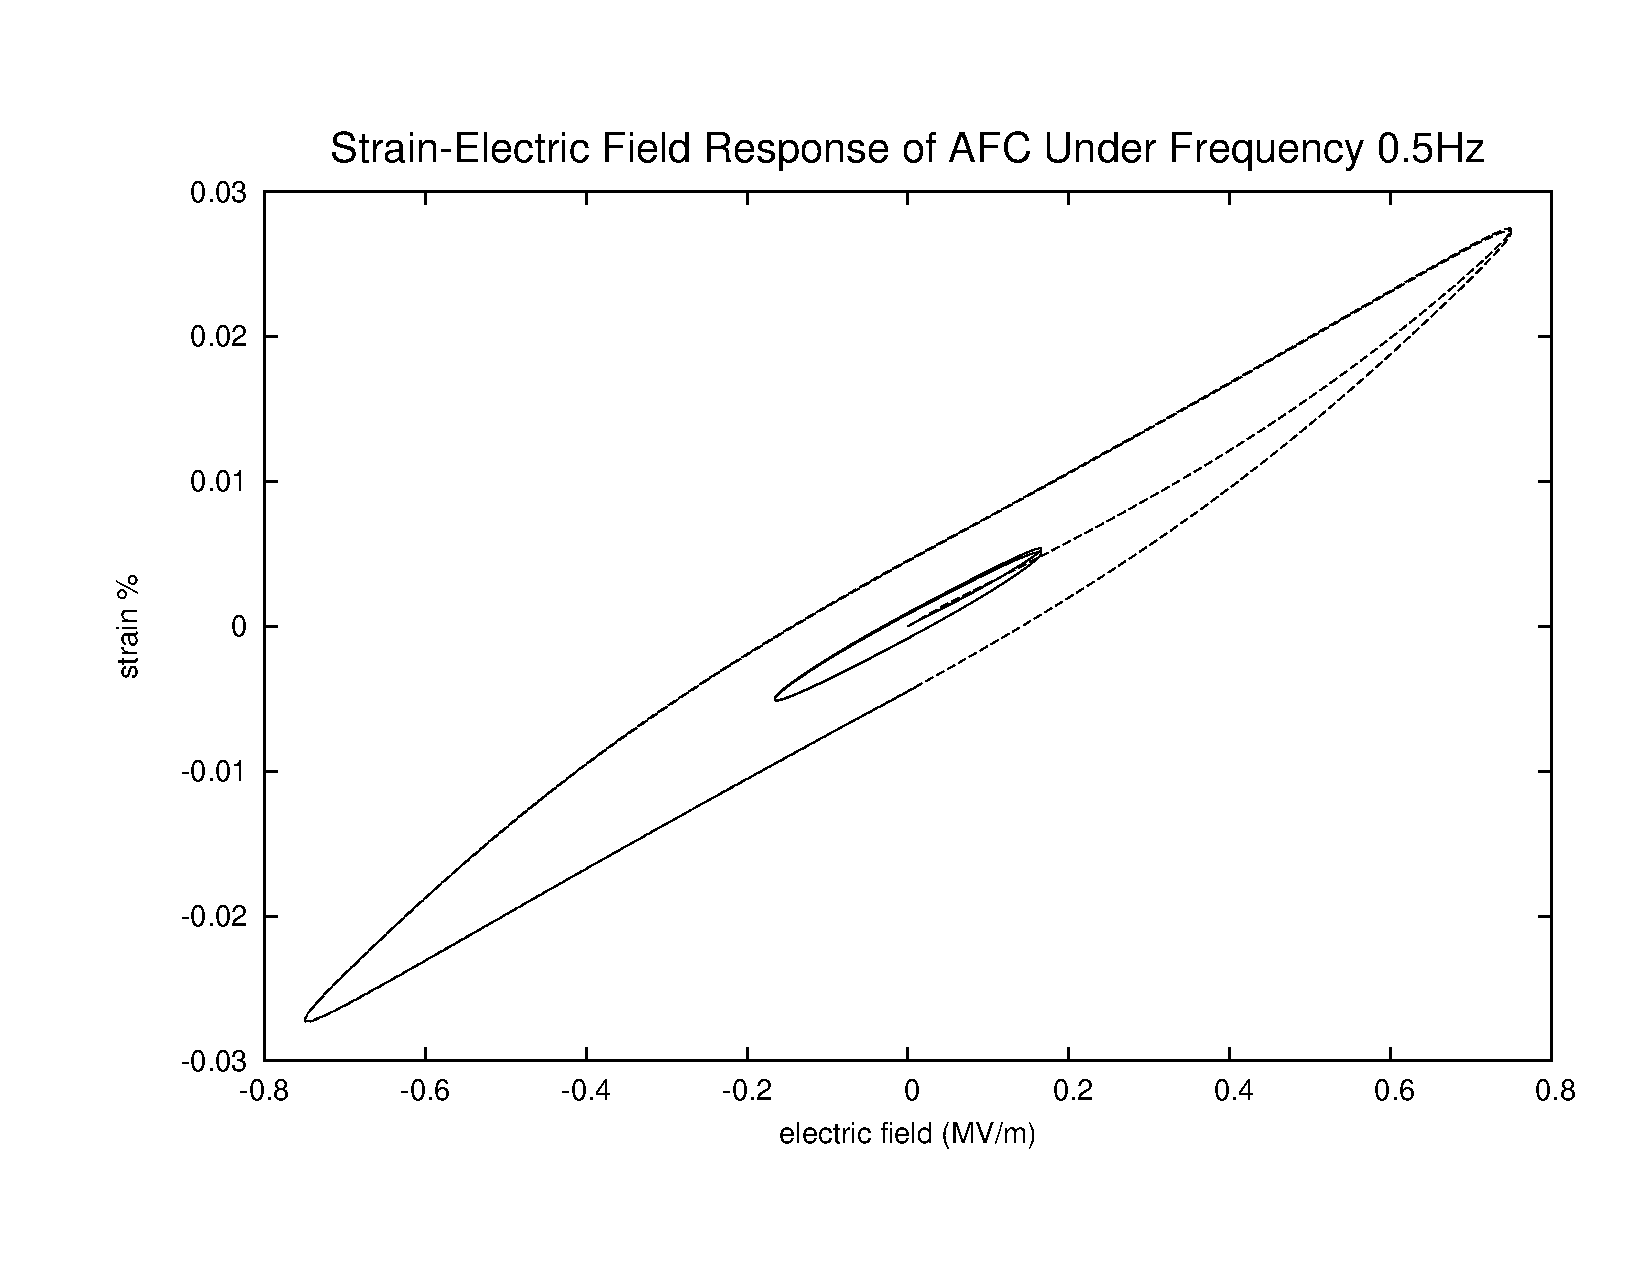
\includegraphics[width=2.5in]{./chap_4_structural_analyses/afc_unit_cell/frequency_effect/electric_field_vs_strains_freq_0p5}}
\subcaptionbox{Frequency 1.0 Hz}
{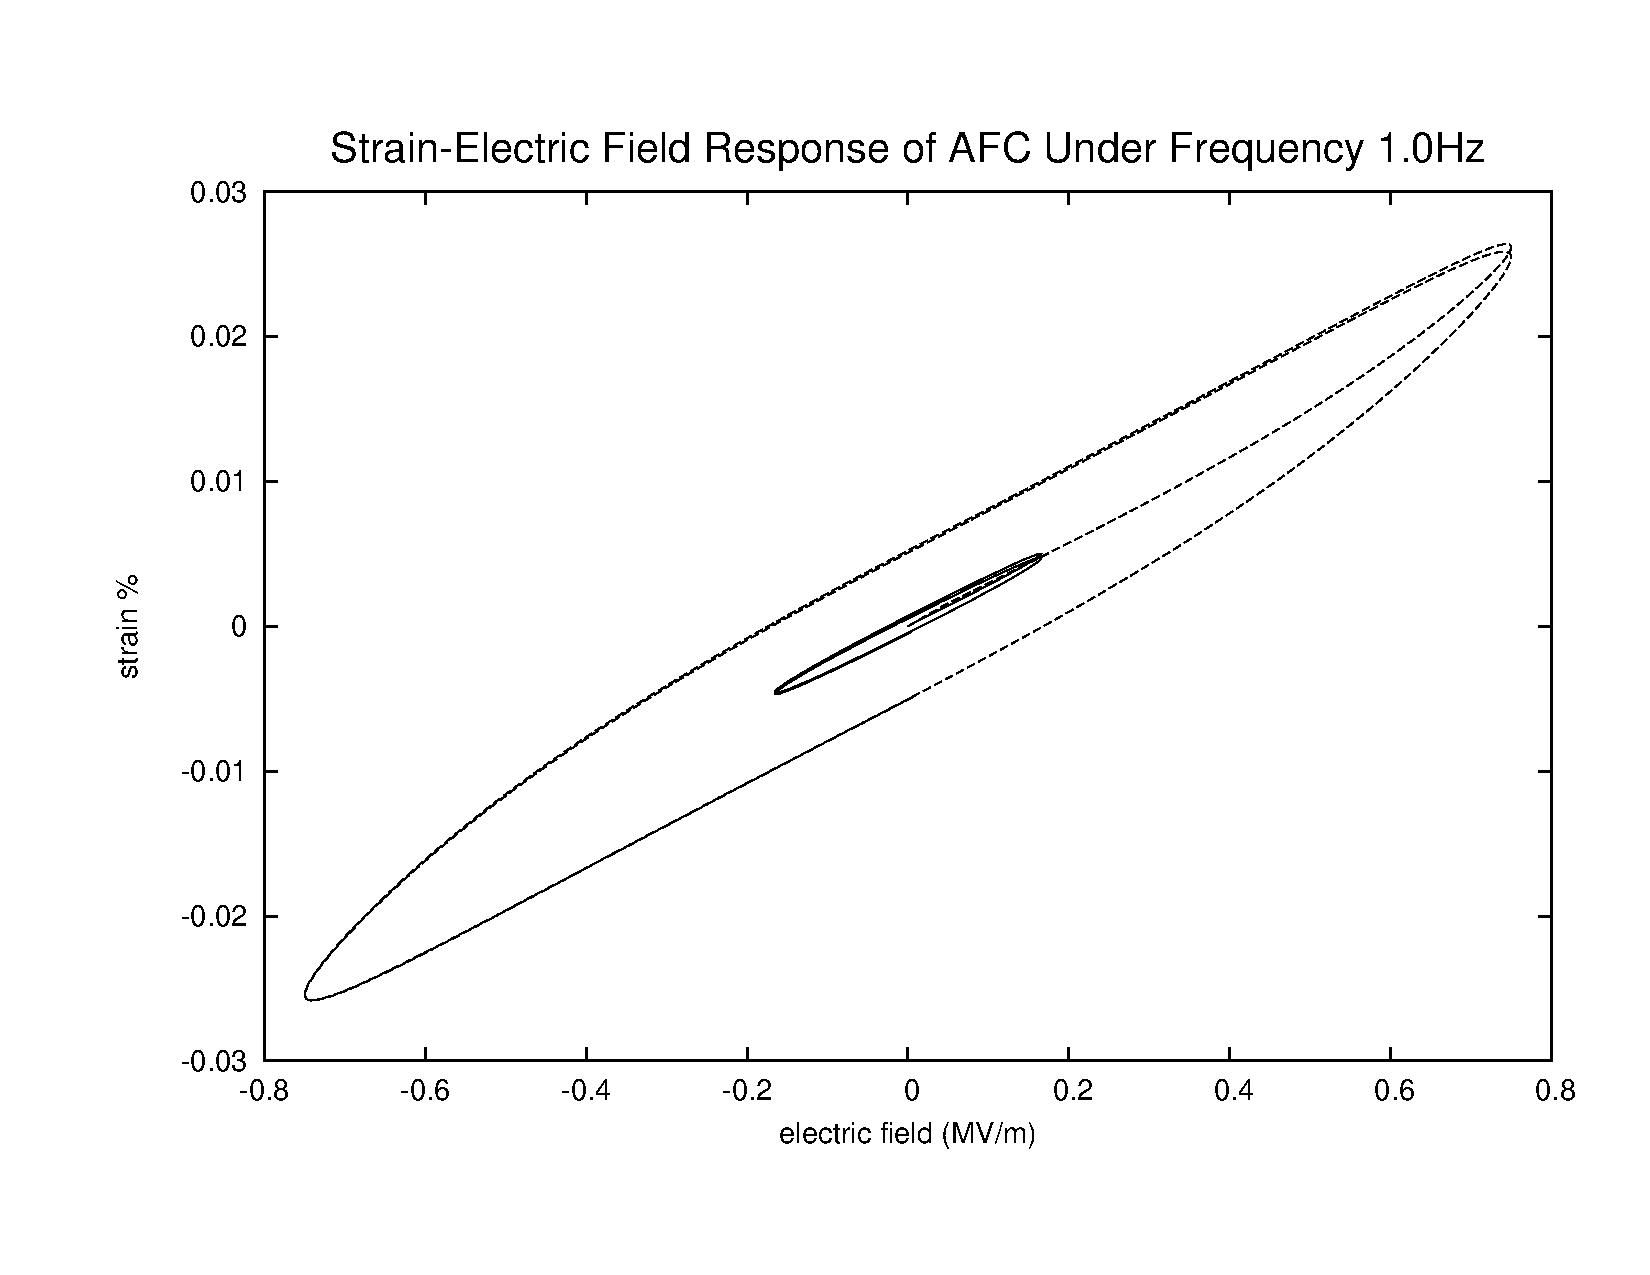
\includegraphics[width=2.5in]{./chap_4_structural_analyses/afc_unit_cell/frequency_effect/electric_field_vs_strains_freq_1p0}}
\subcaptionbox{Frequency 5.0 Hz}
{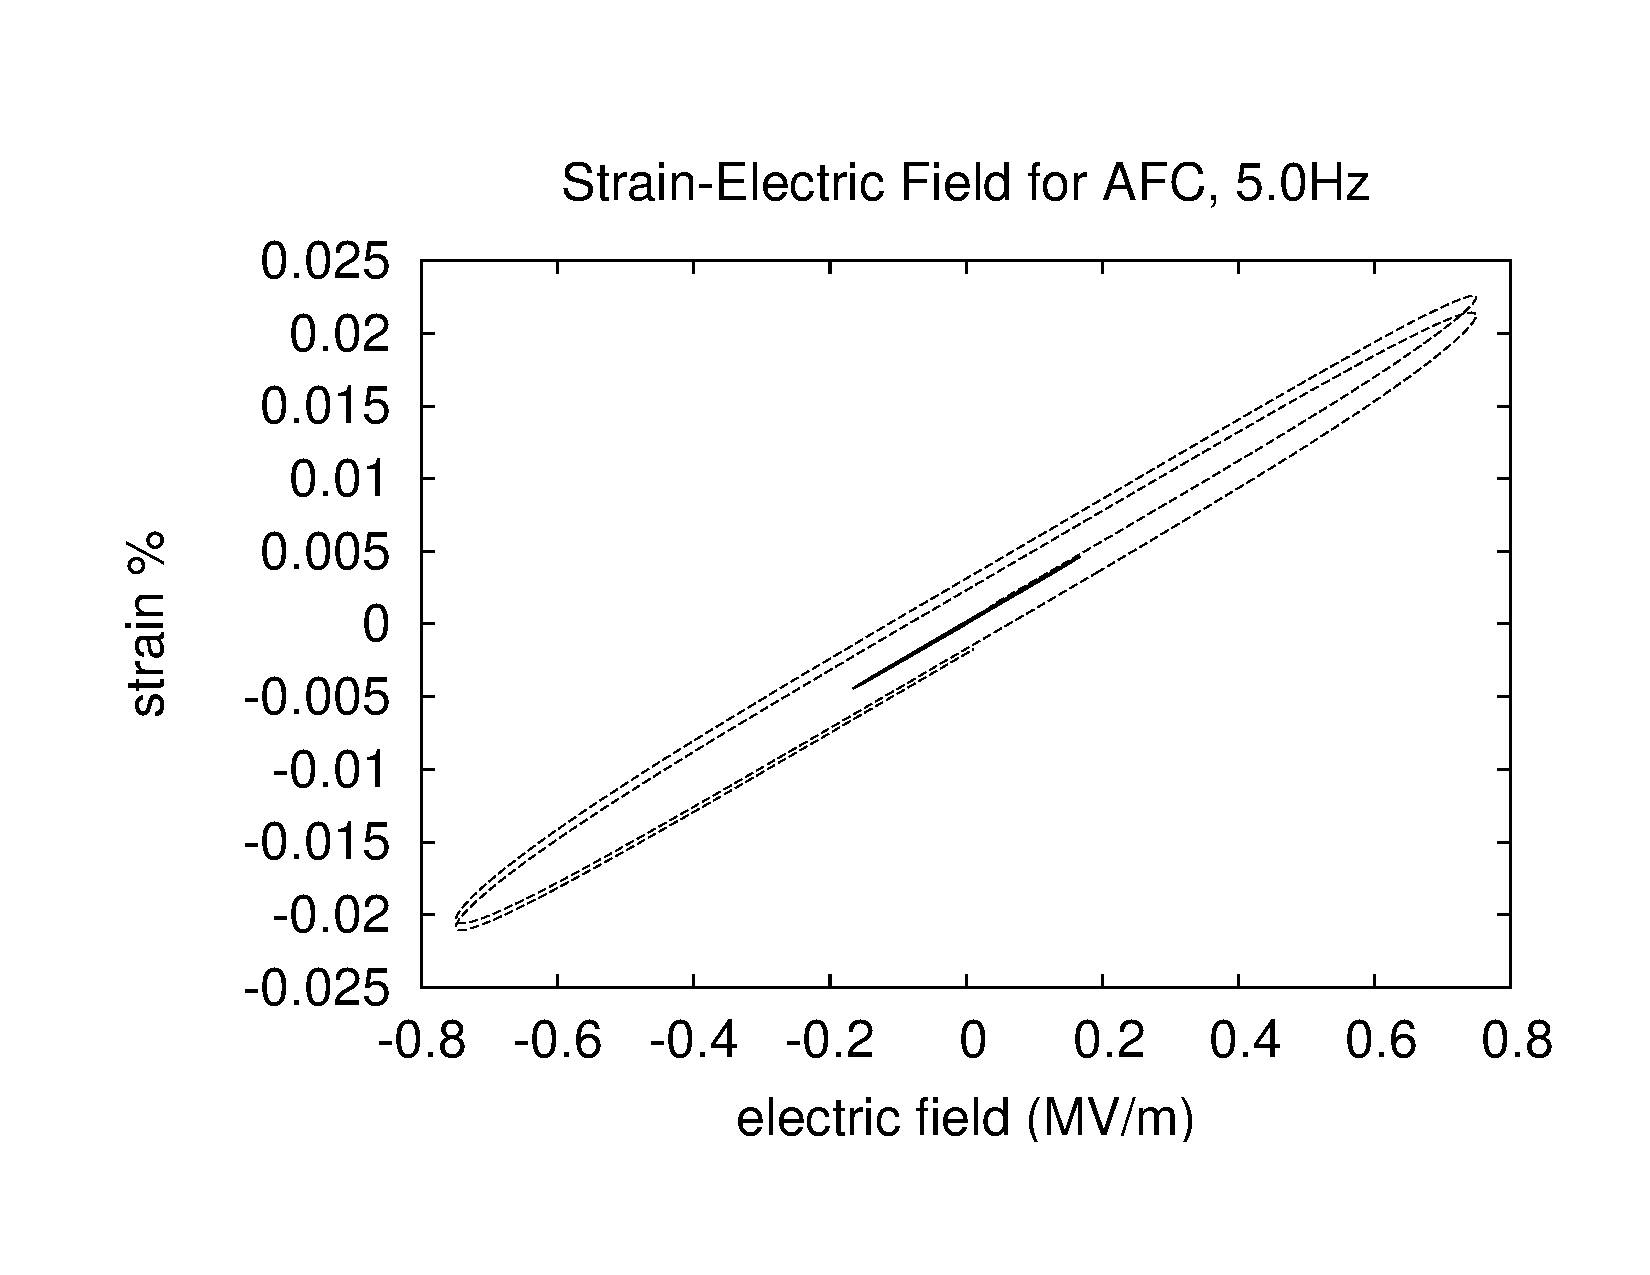
\includegraphics[width=2.5in]{./chap_4_structural_analyses/afc_unit_cell/frequency_effect/electric_field_vs_strains_freq_5p0}}
\subcaptionbox{Frequency 10.0 Hz}
{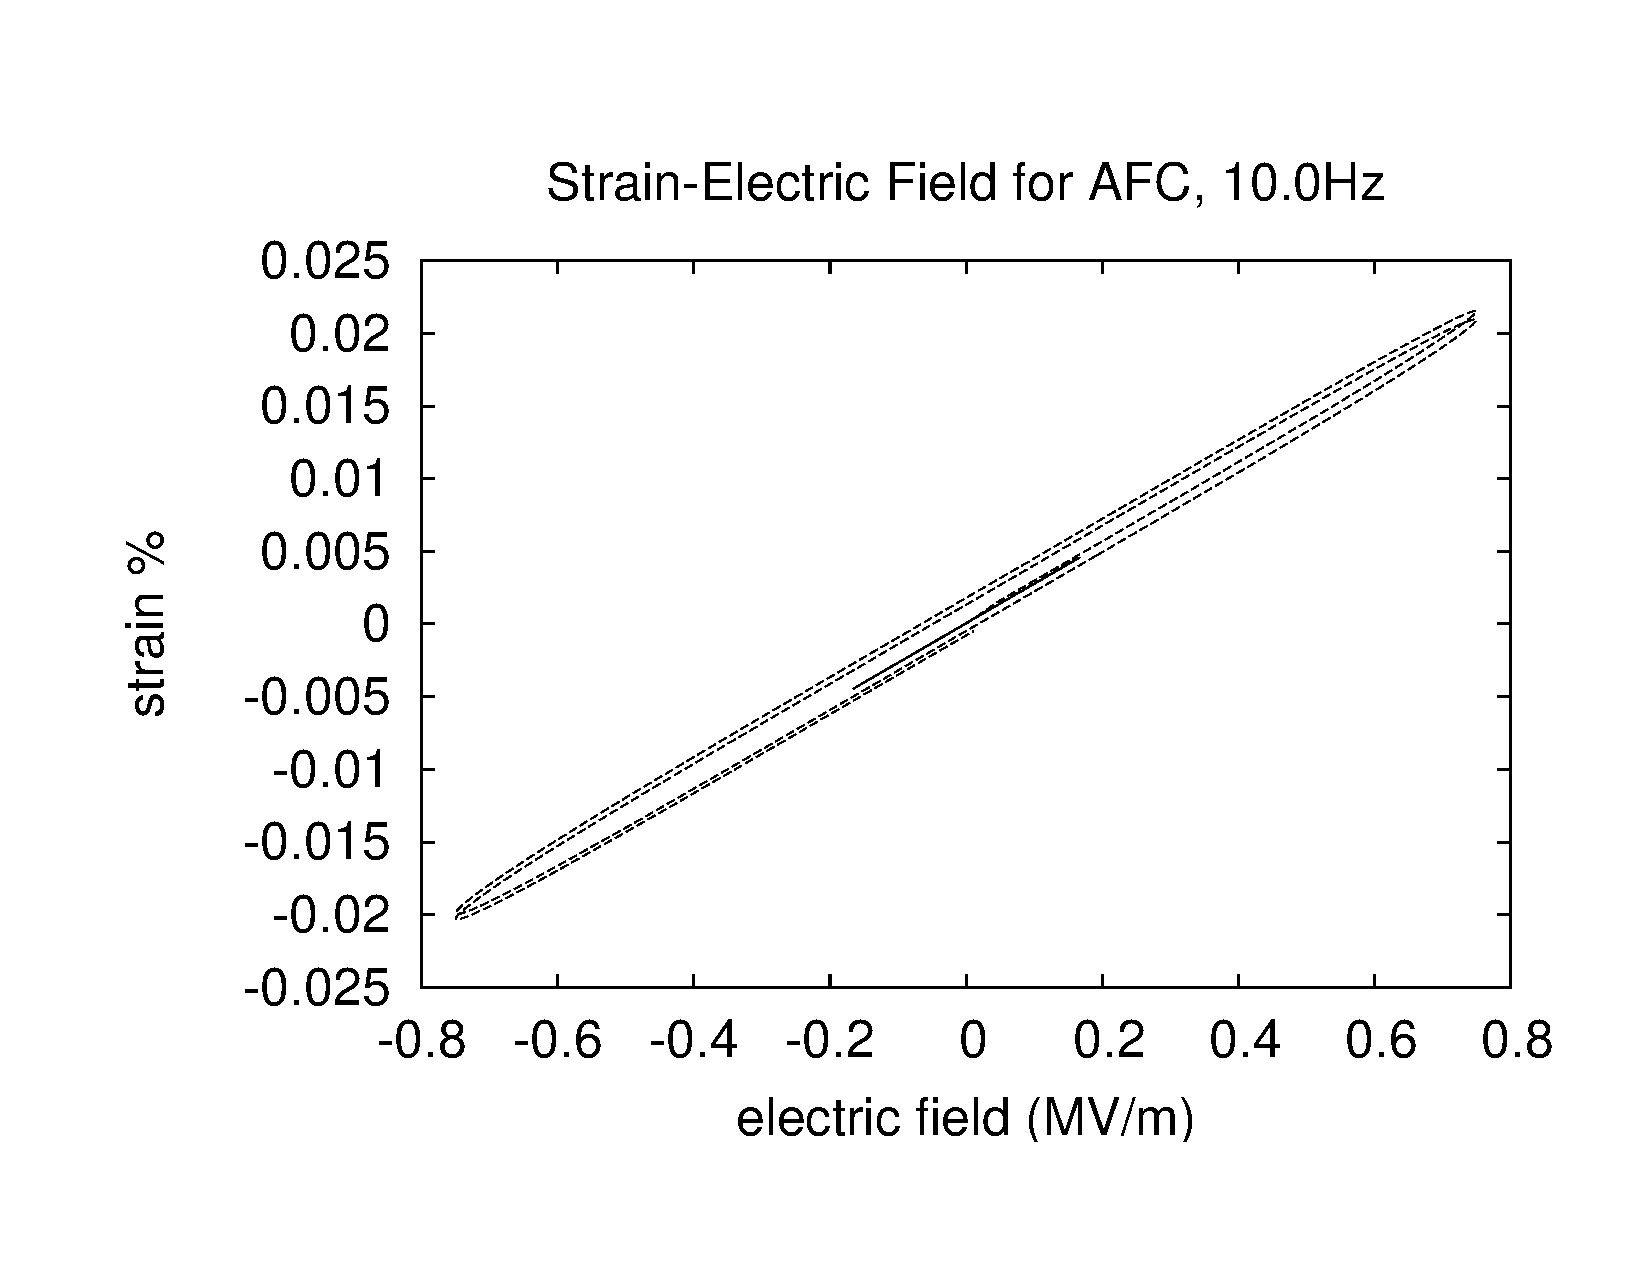
\includegraphics[width=2.5in]{./chap_4_structural_analyses/afc_unit_cell/frequency_effect/electric_field_vs_strains_freq_10p0}}
\caption{Effect of frequency of applied electric field on strain response of AFC}
\label{fig:afc_Frequency_Effect}
\end{figure}
 



\clearpage